% Options for packages loaded elsewhere
\PassOptionsToPackage{unicode}{hyperref}
\PassOptionsToPackage{hyphens}{url}
%
\documentclass[
]{book}
\usepackage{amsmath,amssymb}
\usepackage{lmodern}
\usepackage{iftex}
\ifPDFTeX
  \usepackage[T1]{fontenc}
  \usepackage[utf8]{inputenc}
  \usepackage{textcomp} % provide euro and other symbols
\else % if luatex or xetex
  \usepackage{unicode-math}
  \defaultfontfeatures{Scale=MatchLowercase}
  \defaultfontfeatures[\rmfamily]{Ligatures=TeX,Scale=1}
\fi
% Use upquote if available, for straight quotes in verbatim environments
\IfFileExists{upquote.sty}{\usepackage{upquote}}{}
\IfFileExists{microtype.sty}{% use microtype if available
  \usepackage[]{microtype}
  \UseMicrotypeSet[protrusion]{basicmath} % disable protrusion for tt fonts
}{}
\makeatletter
\@ifundefined{KOMAClassName}{% if non-KOMA class
  \IfFileExists{parskip.sty}{%
    \usepackage{parskip}
  }{% else
    \setlength{\parindent}{0pt}
    \setlength{\parskip}{6pt plus 2pt minus 1pt}}
}{% if KOMA class
  \KOMAoptions{parskip=half}}
\makeatother
\usepackage{xcolor}
\usepackage{longtable,booktabs,array}
\usepackage{calc} % for calculating minipage widths
% Correct order of tables after \paragraph or \subparagraph
\usepackage{etoolbox}
\makeatletter
\patchcmd\longtable{\par}{\if@noskipsec\mbox{}\fi\par}{}{}
\makeatother
% Allow footnotes in longtable head/foot
\IfFileExists{footnotehyper.sty}{\usepackage{footnotehyper}}{\usepackage{footnote}}
\makesavenoteenv{longtable}
\usepackage{graphicx}
\makeatletter
\def\maxwidth{\ifdim\Gin@nat@width>\linewidth\linewidth\else\Gin@nat@width\fi}
\def\maxheight{\ifdim\Gin@nat@height>\textheight\textheight\else\Gin@nat@height\fi}
\makeatother
% Scale images if necessary, so that they will not overflow the page
% margins by default, and it is still possible to overwrite the defaults
% using explicit options in \includegraphics[width, height, ...]{}
\setkeys{Gin}{width=\maxwidth,height=\maxheight,keepaspectratio}
% Set default figure placement to htbp
\makeatletter
\def\fps@figure{htbp}
\makeatother
\setlength{\emergencystretch}{3em} % prevent overfull lines
\providecommand{\tightlist}{%
  \setlength{\itemsep}{0pt}\setlength{\parskip}{0pt}}
\setcounter{secnumdepth}{5}
\usepackage{booktabs}
\ifLuaTeX
  \usepackage{selnolig}  % disable illegal ligatures
\fi
\usepackage[]{natbib}
\bibliographystyle{apalike}
\IfFileExists{bookmark.sty}{\usepackage{bookmark}}{\usepackage{hyperref}}
\IfFileExists{xurl.sty}{\usepackage{xurl}}{} % add URL line breaks if available
\urlstyle{same} % disable monospaced font for URLs
\hypersetup{
  pdftitle={Manual para personas usuarias},
  pdfauthor={Conabio. 2023. Manual para personas usuarias del Sistema Nacional de Información para la Restauración Ambiental, Comisión Nacional para el Conocimiento y Uso de la Biodiversidad. México},
  hidelinks,
  pdfcreator={LaTeX via pandoc}}

\title{Manual para personas usuarias}
\author{Conabio. 2023. Manual para personas usuarias del Sistema Nacional de Información para la Restauración Ambiental, Comisión Nacional para el Conocimiento y Uso de la Biodiversidad. México}
\date{2023-08-30}

\begin{document}
\maketitle

{
\setcounter{tocdepth}{1}
\tableofcontents
}
\hypertarget{snira}{%
\chapter*{SNIRA}\label{snira}}
\addcontentsline{toc}{chapter}{SNIRA}

\includegraphics[width=6.875in,height=\textheight]{https://raw.githubusercontent.com/AngelicaEMB/PruebasManualSNIRA/main/images/CoverPic_Manual.PNG}

El Sistema Nacional de Información para la Restauración Ambiental \href{https://snira.conabio.gob.mx/}{SNIRA} es una plataforma web que integra y sintetiza información relacionada con iniciativas y proyectos de restauración ambiental en el país. El término de `restauración ambiental' se usa para abarcar todas las intervenciones, acciones y trabajos que buscan revertir o reducir las condiciones de degradación, daño o destrucción de los ecosistemas. Por lo tanto, en el SNIRA se incluyen proyectos sobre regeneración natural, restauración ecológica, rehabilitación, restauración productiva, reforestación, refaunación y remediación. Para mayor información al respecto, por favor consulte el documento de \href{https://drive.google.com/file/d/1jmIbkg1UEZI-FfwHULiqkg-rUJExKsIc/view}{\textbf{Enfoques y términos}}.

El SNIRA es un sistema de información de libre acceso a todo público, diseñado con el propósito de reunir y compartir aspectos clave sobre los proyectos de restauración, incluyendo las lecciones aprendidas con el fin de fortalecer la toma de decisiones para el desarrollo sustentable. El sistema permite realizar consultas de la información registrada en la base de datos y agregar información de nuevos proyectos. Para mantener actualizada la información de las iniciativas de restauración, se invita a todas las personas que participaron o están participando en proyectos que revisen si sus proyectos ya fueron incluidos en la base de datos (véase la pestaña `Consulte los proyectos' y la sección `Base de datos'). En caso de no encontrar los proyectos, la persona usuaria puede ingresar la información de proyectos de restauración en proceso de planeación, implementación o concluidos.

\textbf{Si tiene dudas, comentarios sobre el sistema o problemas de navegación, por favor escriba a \href{mailto:snira@conabio.gob.mx}{\nolinkurl{snira@conabio.gob.mx}}}.

\hypertarget{descripciuxf3n-de-la-plataforma}{%
\chapter*{Descripción de la plataforma}\label{descripciuxf3n-de-la-plataforma}}
\addcontentsline{toc}{chapter}{Descripción de la plataforma}

La base de datos del SNIRA está estructurada en cuatro secciones que comprenden 88 campos, de los cuales 33 son campos obligatorios marcados con un asterisco ({*}) que incluye datos acerca de la información general del proyecto, las personas e instituciones involucradas, información relevante sobre diversos aspectos sociales y ambientales y fuentes de información.

En la medida de lo posible, los campos de captura incluyen catálogos de vocabulario controlado para estandarizar la información ingresada en la base de datos. La lista de nombres de especies proviene de los Catálogos de Autoridades Taxonómicas del Sistema Nacional de Información sobre Biodiversidad de México (\url{https://www.snib.mx/}) para evitar posibles errores en su escritura, así como para identificar sinonimias. Las referencias bibliográficas que permiten respaldar la información de la base de datos están directamente vinculadas con los proyectos. A la fecha, se han recopilado 1,600 documentos enfocados al tema de la restauración en México, publicados a partir de 1990. Los documentos incluyen libros, secciones de libros, artículos de revistas científicas y de divulgación, informes, tesis, entre varios otros documentos. La información de estas publicaciones está en proceso de ser capturada en la base de datos.

La información capturada en el SNIRA será revisada por el equipo de trabajo a cargo del SNIRA en la Conabio para evitar inconsistencias y asegurar en la medida de lo posible la calidad de los datos. Una vez que el proyecto haya sido revisado y aprobado, la información estará disponible para su consulta por parte del público en general.

\textbf{Si tiene dudas, comentarios sobre el sistema o problemas de navegación, por favor escriba a \href{mailto:snira@conabio.gob.mx}{\nolinkurl{snira@conabio.gob.mx}}}.

\hypertarget{instrucciones-generales}{%
\chapter*{Instrucciones generales}\label{instrucciones-generales}}
\addcontentsline{toc}{chapter}{Instrucciones generales}

La base de datos del SNIRA comprende cuatro secciones y 88 campos, de los cuales {\textbf{33 son campos obligatorios marcados con un asterisco (*)}} que son imprescindibles llenarlos.

Se recomienda agregar toda la información disponible con la finalidad de enriquecer al SNIRA y apoyar al cumplimiento de los objetivos para los que fue diseñado.

En la medida de lo posible, los campos incluyen catálogos de vocabulario controlado para facilitar la captura de información y estandarizar las respuestas en la base de datos. Por favor, seleccione la opción de respuesta que más se ajuste a su proyecto. En caso de no contar con información para un campo, por favor seleccione `No determinado'. Si el campo no aplica para su proyecto, por favor seleccione `No aplica'.

Si no encuentra una opción de respuesta que aplique a su proyecto, puede escribir su respuesta en los campos de texto abierto correspondientes, estos campos sirven para poder proporcionar mayor detalle o escribir comentarios. Los campos de texto abierto se encuentran en todas las secciones y subsecciones del sistema.

Por favor, escriba y capture los datos en español. Si copia información de un documento, póngala entre comillas ('' ``) para indicar que es una cita textual. Si la información está en un idioma distinto al español, favor de traducirla; se puede usar el servicio de traducción como \href{https://translate.google.com.mx/?hl=es}{Google}, \href{https://www.deepl.com/es/translator}{DeepL} u otro para apoyar con la traducción de textos al español. En caso de usar un servicio de traducción, favor de indicar al final del texto lo siguiente: 'Traducido por XX´.

\begin{center}\rule{0.5\linewidth}{0.5pt}\end{center}

\hypertarget{guardar-informaciuxf3n-capturada}{%
\section*{Guardar información capturada}\label{guardar-informaciuxf3n-capturada}}
\addcontentsline{toc}{section}{Guardar información capturada}

Después de capturar los datos de cada sección y subsección, pulse `Guardar' para almacenar la información ingresada. Si todos los campos obligatorios han sido llenados, el sistema abrirá una ventana con la leyenda `Cambios guardados'. Pulse el botón `Aceptar' para asegurar que la información se ha guardado en el sistema. El botón de `Guardar' solamente se activará cuando todos los campos obligatorios de una sección tengan información. \textbf{Si por algún motivo tiene que interrumpir el llenado de campos, asegúrese de llenar todos los campos obligatorios y pulsar el botón `Guardar' para poder seguir la captura en otro momento}.

Pulse el botón `Siguiente' para pasar a la siguiente sección o subsección.

\begin{center}\rule{0.5\linewidth}{0.5pt}\end{center}

\hypertarget{editar-informaciuxf3n-capturada}{%
\section*{Editar información capturada}\label{editar-informaciuxf3n-capturada}}
\addcontentsline{toc}{section}{Editar información capturada}

Podrá editar la información las veces que sean necesarias mientras su proyecto esté en el estado de \textbf{`Edición'} (véase las `Instrucciones' en la parte superior de la sección 1: Información general). Una vez que pulse el botón `Enviar a revisión mi proyecto' (ubicado al final de los campos, es decir después la sección 4: Fuentes de información), automáticamente el estado del proyecto cambiará a `En revisión' y ya no será posible hacer cambios. En caso de que haya campos obligatorios vacíos o el sistema encuentra inconsistencias en los datos capturados, el estado se mantendrá en `Edición'. \textbf{Si requiere hacer algún cambio después de haber enviado el proyecto a revisión, deberá enviar un correo electrónico a \href{mailto:snira@conabio.gob.mx}{\nolinkurl{snira@conabio.gob.mx}}}

La información de su proyecto estará disponible para la consulta del público en general cuando los datos hayan sido revisados por el equipo de trabajo de la Conabio y el proyecto se haya registrado en la base de datos del SNIRA. En ese caso, el estatus del proyecto cambiará a `REGISTRADO'.

A continuación se explican con detalle cada una de las secciones y los campos del SNIRA, además se proporcionan algunos ejemplos para la captura de información.

\begin{center}\rule{0.5\linewidth}{0.5pt}\end{center}

\hypertarget{primer-paso}{%
\section*{Primer paso}\label{primer-paso}}
\addcontentsline{toc}{section}{Primer paso}

\textbf{Registre un nuevo proyecto}
En esta sección encontrará las instrucciones para la captura de la información en la base de datos, así como el \href{https://www.biodiversidad.gob.mx/conabio/proteccion-DP/ap-solicitudes-de-acceso-infopub}{\textbf{Aviso de privacidad}} y los \href{https://www.gob.mx/terminos}{\textbf{Términos y condiciones de uso del sitio}}.

El primer campo obligatorio es `Nombre del proyecto'. Al escribir el nombre (en español) y pulsar el botón `Crear nuevo proyecto', se habilitarán los demás campos para ingresar la información de su proyecto. Cuando la información que se captura es extraída de una publicación, ponga el título de la publicación.

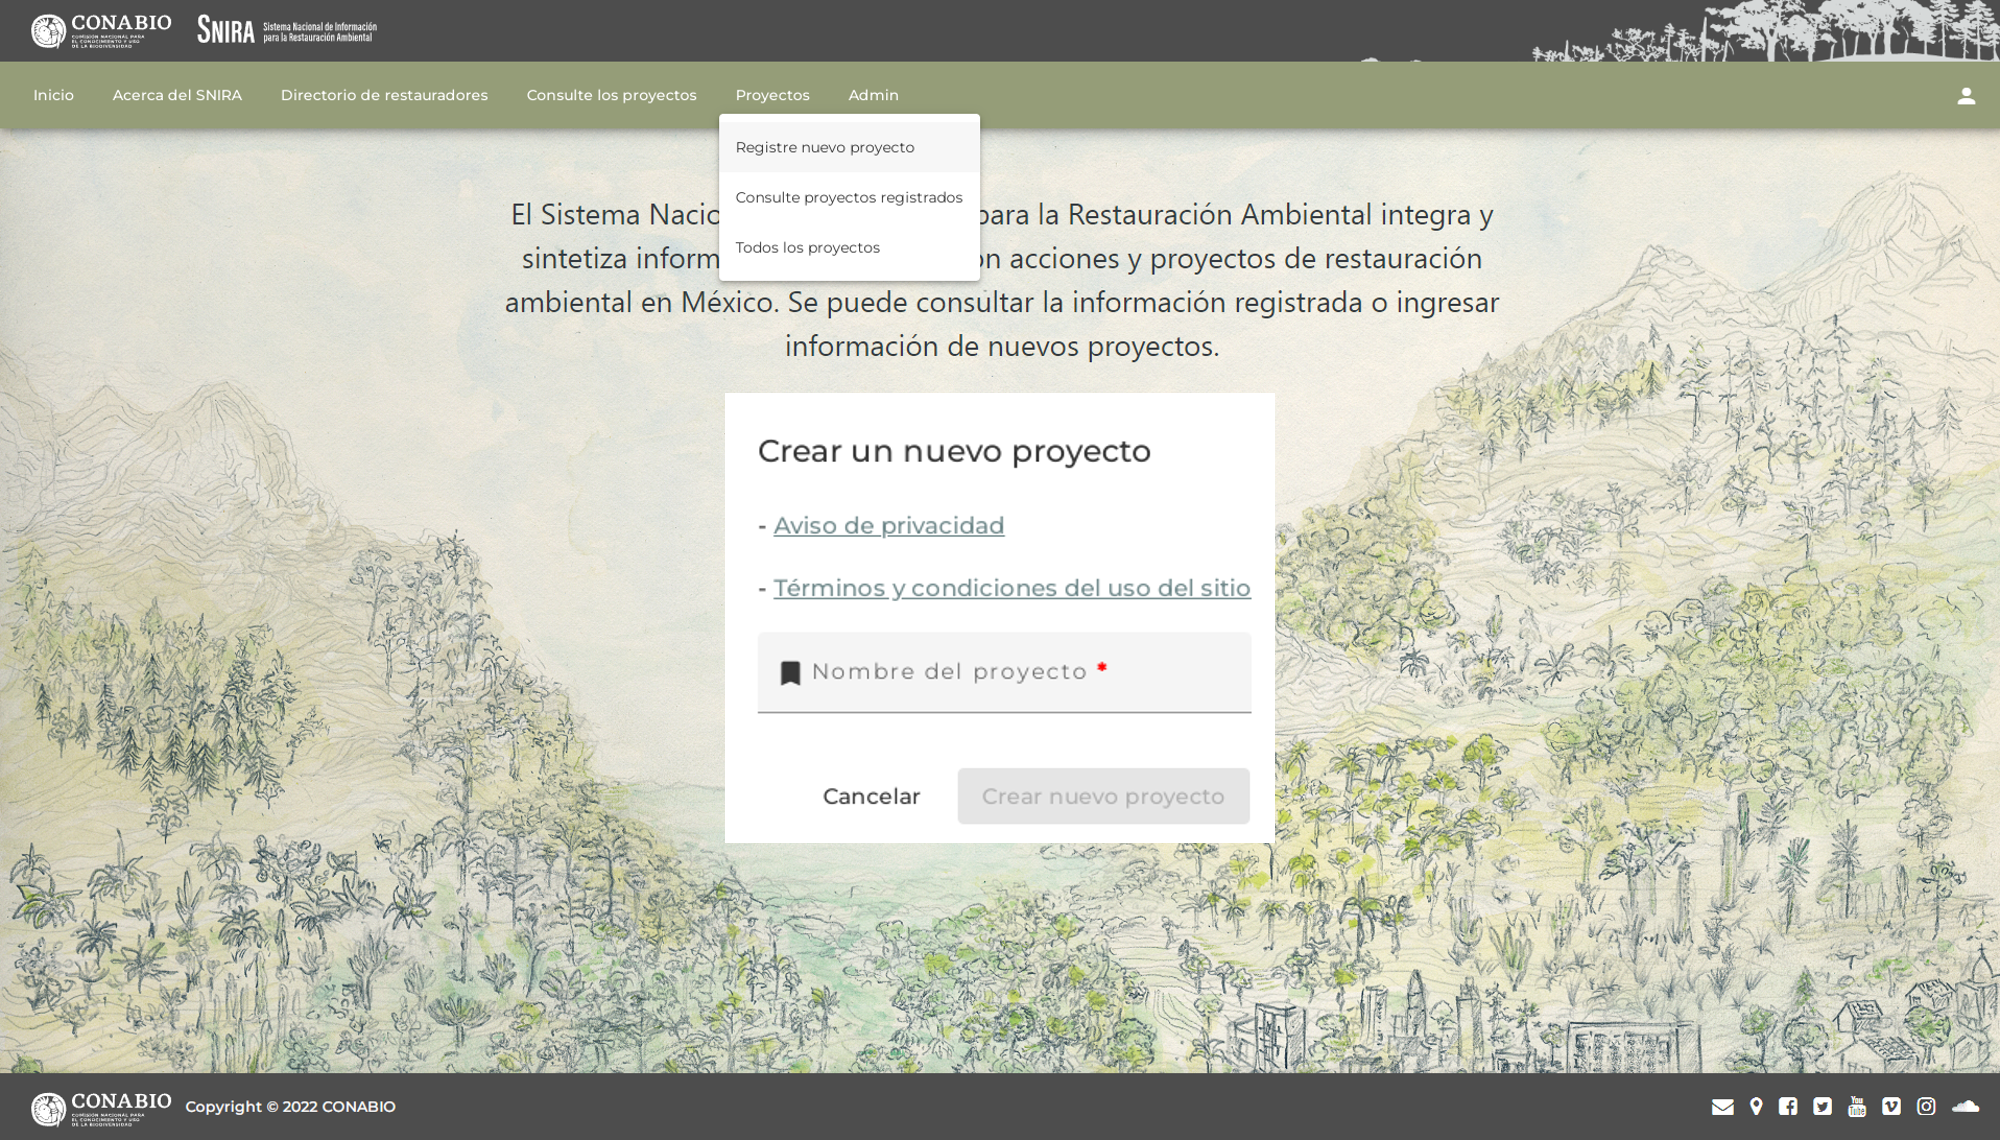
\includegraphics[width=6.77083in,height=\textheight]{https://raw.githubusercontent.com/AngelicaEMB/PruebasManualSNIRA/main/images/Imagen1.png}

\begin{center}\rule{0.5\linewidth}{0.5pt}\end{center}

\hypertarget{ventana-de-inicio}{%
\section*{Ventana de inicio}\label{ventana-de-inicio}}
\addcontentsline{toc}{section}{Ventana de inicio}

Después de ingresar el nombre del proyecto, mismo que podrá editar posteriormente si así lo desea, aparecerá la ventana principal donde podrá navegar entre secciones

\includegraphics[width=7.29167in,height=\textheight]{https://raw.githubusercontent.com/AngelicaEMB/PruebasManualSNIRA/main/images/01_Inicio.png}

\hypertarget{informaciuxf3n-general}{%
\chapter{Información general}\label{informaciuxf3n-general}}

La sección comprende 25 campos, de los cuales \textbf{7 son obligatorios} ({*}).

Los campos de `Identificador único' y `Estatus', ubicados en la parte superior, son asignados automáticamente y no pueden ser modificados por las personas usuarias.

\includegraphics[width=5.20833in,height=\textheight]{https://raw.githubusercontent.com/AngelicaEMB/PruebasManualSNIRA/main/images/02_Identificador.png}

\begin{center}\rule{0.5\linewidth}{0.5pt}\end{center}

\hypertarget{nombre-del-proyecto}{%
\subsection*{\texorpdfstring{{Nombre del proyecto*}}{Nombre del proyecto*}}\label{nombre-del-proyecto}}
\addcontentsline{toc}{subsection}{{Nombre del proyecto*}}

Escriba el nombre de un proyecto en español (p.~ej., Programa Nacional para la Conservación y Restauración Integral de las Islas de México). Cuando la información que se captura es extraída de una publicación, ponga el título de la publicación en español.

Si el nombre de la publicación o del proyecto está en un idioma distinto, favor de traducirlo y escribir el nombre original en el siguiente campo ``Nombre original del proyecto''.

\includegraphics[width=7.29167in,height=\textheight]{https://raw.githubusercontent.com/AngelicaEMB/PruebasManualSNIRA/main/images/03_NomProy.png}

\begin{center}\rule{0.5\linewidth}{0.5pt}\end{center}

\hypertarget{nombre-original-del-proyecto}{%
\subsection*{Nombre original del proyecto}\label{nombre-original-del-proyecto}}
\addcontentsline{toc}{subsection}{Nombre original del proyecto}

Escriba el nombre de un proyecto en el idioma original cuando este sea diferente al español. Cuando la información que se captura es extraída de una publicación, ponga el título de la publicación.

En caso de que el título de la publicación esté en español, no es necesario repetirlo; sólo quedará en el campo ``Nombre del proyecto''.

\begin{center}\rule{0.5\linewidth}{0.5pt}\end{center}

\hypertarget{tipo-de-proyecto}{%
\subsection*{\texorpdfstring{{Tipo de proyecto*}}{Tipo de proyecto*}}\label{tipo-de-proyecto}}
\addcontentsline{toc}{subsection}{{Tipo de proyecto*}}

Seleccione la opción que corresponda:

\begin{itemize}
\tightlist
\item
  Teórico: Hace referencia a proyectos de experimentación en laboratorio o vivero, revisión de literatura, meta-análisis, entrevistas, modelación, desarrollo de plan de manejo, entre otros.
\item
  Práctico: Hace referencia a proyectos que implementan acciones de restauración campo.
\item
  Teórico-Práctico: Hace referencia a proyectos mixtos, p.~ej., germinación y crecimiento en invernadero y posterior trasplante a campo.
\end{itemize}

\begin{center}\rule{0.5\linewidth}{0.5pt}\end{center}

\hypertarget{el-proyecto-forma-parte-de-un-proyecto-muxe1s-amplio}{%
\subsection*{\texorpdfstring{{¿El proyecto forma parte de un proyecto más amplio?*}}{¿El proyecto forma parte de un proyecto más amplio?*}}\label{el-proyecto-forma-parte-de-un-proyecto-muxe1s-amplio}}
\addcontentsline{toc}{subsection}{{¿El proyecto forma parte de un proyecto más amplio?*}}

Seleccione la opción que corresponda:

\begin{itemize}
\item
  No: Refiere a un proyecto que se registra de forma individual y hasta donde se sabe no forma parte de un proyecto general (p.~ej., Restoration planning to guide Aichi targets in a megadiverse country).
\item
  Sí: Refiere a un programa o proyecto general que incluye proyectos específicos (p.~ej., Proyecto GEF-Invasoras `Aumentar las Capacidades Nacionales para el Manejo de las Especies Exóticas Invasoras (EEI) a través de la Implementación de la Estrategia Nacional de EEI' o Programas de Acción para la Conservación de Especie (PACE)).
\end{itemize}

En caso de que sí forme parte de un proyecto más amplio, seleccione la opción que corresponda de la lista.

\begin{center}\rule{0.5\linewidth}{0.5pt}\end{center}

\hypertarget{seleccione-el-nombre-del-proyecto-muxe1s-amplio}{%
\subsubsection*{Seleccione el nombre del proyecto más amplio}\label{seleccione-el-nombre-del-proyecto-muxe1s-amplio}}
\addcontentsline{toc}{subsubsection}{Seleccione el nombre del proyecto más amplio}

Seleccione la opción de la lista que corresponda. Si el nombre del proyecto no aparece en la lista, favor de capturarlo en el siguiente campo.

\includegraphics[width=6.875in,height=\textheight]{https://raw.githubusercontent.com/AngelicaEMB/PruebasManualSNIRA/main/images/05.2_ProyeAmplio.png}

\begin{center}\rule{0.5\linewidth}{0.5pt}\end{center}

\hypertarget{escriba-el-nombre-del-proyecto-cuando-no-aparece-en-la-lista}{%
\subsubsection*{Escriba el nombre del proyecto cuando no aparece en la lista}\label{escriba-el-nombre-del-proyecto-cuando-no-aparece-en-la-lista}}
\addcontentsline{toc}{subsubsection}{Escriba el nombre del proyecto cuando no aparece en la lista}

Campo de texto abierto que permite introducir el nombre del proyecto más amplio o si el proyecto está ligado a dos o más proyectos generales.

\includegraphics[width=6.875in,height=\textheight]{https://raw.githubusercontent.com/AngelicaEMB/PruebasManualSNIRA/main/images/05.3_ProyeAmplio.png}

\begin{center}\rule{0.5\linewidth}{0.5pt}\end{center}

\hypertarget{objetivo-del-proyecto}{%
\subsection*{\texorpdfstring{{Objetivo del proyecto*}}{Objetivo del proyecto*}}\label{objetivo-del-proyecto}}
\addcontentsline{toc}{subsection}{{Objetivo del proyecto*}}

Escriba el objetivo general del proyecto y los particulares en caso que aplique. Si copia el objetivo de una publicación, póngalo entre comillas '' '' para indicar que es una cita textual.

Si los objetivos están en un idioma distinto al español, favor de traducirlos. Puede usar un servicio de traducción en línea (p.ej., Traductor de \href{https://translate.google.com.mx/?hl=es}{Google} o \href{https://www.deepl.com/es/translator}{DeepL}), en caso de usar un servicio de traducción favor de indicar al final del resumen lo siguiente: 'Traducido por XX´.

\includegraphics[width=7.29167in,height=\textheight]{https://raw.githubusercontent.com/AngelicaEMB/PruebasManualSNIRA/main/images/06_ObjProy.png}

\begin{center}\rule{0.5\linewidth}{0.5pt}\end{center}

\hypertarget{enfoque-del-proyecto-seguxfan-la-persona-usuaria}{%
\subsection*{Enfoque del proyecto según la persona usuaria}\label{enfoque-del-proyecto-seguxfan-la-persona-usuaria}}
\addcontentsline{toc}{subsection}{Enfoque del proyecto según la persona usuaria}

El enfoque se refiere al planteamiento general de su proyecto, p.~ej., recuperación del suelo; plantación experimental con fines de restauración. El enfoque es establecido por el criterio y conocimiento de la persona usuaria.

Para información recabada a partir de una publicación, indique el enfoque o término usado en la publicación.
El enfoque o término capturado puede ser el mismo que se indique en el campo `Enfoque del proyecto según el SNIRA'.

\includegraphics[width=7.29167in,height=\textheight]{https://raw.githubusercontent.com/AngelicaEMB/PruebasManualSNIRA/main/images/Imagen2.png}

\begin{center}\rule{0.5\linewidth}{0.5pt}\end{center}

\hypertarget{enfoque-del-proyecto-seguxfan-el-snira}{%
\subsection*{\texorpdfstring{{Enfoque del proyecto según el SNIRA*}}{Enfoque del proyecto según el SNIRA*}}\label{enfoque-del-proyecto-seguxfan-el-snira}}
\addcontentsline{toc}{subsection}{{Enfoque del proyecto según el SNIRA*}}

Seleccione la opción que corresponda.
Consulte el documento \href{https://drive.google.com/file/d/1jmIbkg1UEZI-FfwHULiqkg-rUJExKsIc/view}{\textbf{Enfoques y términos}} para más información.

\begin{itemize}
\tightlist
\item
  Regeneración natural: Proceso natural en áreas que pueden recuperar o restablecer por sí solas su estructura y composición florística (al menos parcialmente).
  Los niveles de degradación generalmente son bajos, por lo que no se requiere intervención o los niveles de intervención son mínimos para reducir los factores de presión y amenaza.
\item
  Restauración ecológica: Conjunto de acciones que buscan el máximo nivel de recuperación de las áreas degradadas.
  Las acciones están enfocadas a recuperar los componentes, funciones y procesos de los ecosistemas degradados para contribuir a la conservación de la biodiversidad y la provisión de servicios ambientales.
\item
  Rehabilitación: Conjunto de acciones dirigidas a recuperar ciertos componentes o atributos de los ecosistemas degradados, frecuentemente asociados a su funcionalidad y a la provisión de servicios ambientales, p.~ej., la composición biótica, estructura de la vegetación o alguna función del ecosistema.
\item
  Restauración productiva: Conjunto de acciones que fortalecen e impulsan el desarrollo de actividades productivas sustentables, p.~ej., por medio de prácticas agroecológicas, sistemas agroforestales y silvicultura.
\item
  Reforestación: Conjunto de actividades tendientes a la rehabilitación parcial o total de las funciones de un ecosistema forestal por medio del establecimiento de especies forestales.
\item
  Refaunación: Conjunto de acciones basadas en el manejo, introducción o reintroducción de poblaciones de fauna silvestre nativa que puedan reinstalar funciones ecológicas en una área, lo cual contribuye a la restauración de los ecosistemas.
\item
  Remediación: Conjunto de actividades que generalmente se emplean en sitios severamente impactados y degradados por actividades antropogénicas, p.~ej., en minas a cielo abierto, vertederos o sitios postindustriales.
  El objetivo principal es controlar o eliminar contaminantes que afectan o perturban en un área la calidad de suelo, agua o aire. Puede resultar en un reemplazo o reconstrucción de un ecosistema original.
\item
  No aplica: Seleccione cuando ninguna de las otras opciones aplica.
\end{itemize}

\includegraphics[width=6.875in,height=\textheight]{https://raw.githubusercontent.com/AngelicaEMB/PruebasManualSNIRA/main/images/08_EnfoSNIRA.png}

\begin{center}\rule{0.5\linewidth}{0.5pt}\end{center}

\hypertarget{comentarios-respecto-al-enfoque-del-proyecto}{%
\subsection*{Comentarios respecto al enfoque del proyecto}\label{comentarios-respecto-al-enfoque-del-proyecto}}
\addcontentsline{toc}{subsection}{Comentarios respecto al enfoque del proyecto}

Campo de texto abierto que permite introducir comentarios o proporcionar mayores detalles respecto al enfoque del proyecto.

\begin{center}\rule{0.5\linewidth}{0.5pt}\end{center}

\hypertarget{resumen-del-proyecto}{%
\subsection*{Resumen del proyecto}\label{resumen-del-proyecto}}
\addcontentsline{toc}{subsection}{Resumen del proyecto}

Por favor, escriba un resumen.
Para información extraída de una publicación, incluya el resumen entre comillas '' '' para indicar que es una cita textual.

Si el resumen está en un idioma distinto al español, favor de traducirlo. Puede usar un servicio de traducción disponible en línea (p.ej. Traductor de \href{https://translate.google.com.mx/?hl=es}{Google} o \href{https://www.deepl.com/es/translator}{DeepL}), favor de indicar que fue 'Traducido por XX´.

\begin{center}\rule{0.5\linewidth}{0.5pt}\end{center}

\hypertarget{palabras-clave}{%
\subsection*{Palabras clave}\label{palabras-clave}}
\addcontentsline{toc}{subsection}{Palabras clave}

Las palabras claves son términos compuestos por una o más palabras que refieren a aspectos particulares o elementos clave de un proyecto para facilitar su clasificación y búsqueda dentro de la base de datos.

Puede capturar hasta cinco palabras clave, p.~ej., `planeación sistemática', `especies exóticas invasoras', `suelos alcalinos', `bioremediación', `fertilización', `plantación de árboles', `análisis multicriterio'.

Para información extraída de una publicación, por favor incluya las palabras clave indicadas en la publicación. Si las palabras clave están en un idioma distinto al español, favor de traducirlas.

\begin{center}\rule{0.5\linewidth}{0.5pt}\end{center}

\hypertarget{auxf1o-de-inicio-del-proyecto}{%
\subsection*{Año de inicio del proyecto}\label{auxf1o-de-inicio-del-proyecto}}
\addcontentsline{toc}{subsection}{Año de inicio del proyecto}

El año de inicio se considera a partir de la fase de planeación del proyecto; si el proyecto no cuenta con fase de planeación, se puede considerar a partir de la fase de implementación.

Seleccione la opción de `----' cuando se desconoce el año de inicio.

\begin{center}\rule{0.5\linewidth}{0.5pt}\end{center}

\hypertarget{mes-de-inicio-del-proyecto}{%
\subsection*{Mes de inicio del proyecto}\label{mes-de-inicio-del-proyecto}}
\addcontentsline{toc}{subsection}{Mes de inicio del proyecto}

El mes de inicio se considera a partir de la fase de planeación del proyecto o bien a partir de la fase de implementación.

Seleccione la opción de `----' cuando se desconoce el mes de inicio.

\begin{center}\rule{0.5\linewidth}{0.5pt}\end{center}

\hypertarget{auxf1o-de-tuxe9rmino-del-proyecto}{%
\subsection*{Año de término del proyecto}\label{auxf1o-de-tuxe9rmino-del-proyecto}}
\addcontentsline{toc}{subsection}{Año de término del proyecto}

El año de término se considera después de la fase de implementación y monitoreo, es decir a la conclusión del proyecto.

Si el proyecto no considera fase de monitoreo o fue cancelado, indique el año en el que se realizaron las últimas acciones del proyecto.

Seleccione la opción de `----' cuando no es posible determinar el año de término.

\begin{center}\rule{0.5\linewidth}{0.5pt}\end{center}

\hypertarget{mes-de-tuxe9rmino-del-proyecto}{%
\subsection*{Mes de término del proyecto}\label{mes-de-tuxe9rmino-del-proyecto}}
\addcontentsline{toc}{subsection}{Mes de término del proyecto}

El mes de término se considera después de la fase de implementación y monitoreo, es decir a la conclusión del proyecto.

Si el proyecto no considera fase de monitoreo o fue cancelado indique el mes en el que se realizaron las últimas acciones del proyecto.

Seleccione la opción de `----' cuando no es posible determinar el mes de término.

\begin{center}\rule{0.5\linewidth}{0.5pt}\end{center}

\hypertarget{etapa-o-fase-en-la-que-se-encuentra-el-proyecto}{%
\subsection*{\texorpdfstring{{Etapa o fase en la que se encuentra el proyecto*}}{Etapa o fase en la que se encuentra el proyecto*}}\label{etapa-o-fase-en-la-que-se-encuentra-el-proyecto}}
\addcontentsline{toc}{subsection}{{Etapa o fase en la que se encuentra el proyecto*}}

Seleccione la opción que corresponda:

\begin{itemize}
\tightlist
\item
  En proceso: El proyecto se encuentra en la fase de planeación, implementación o monitoreo.
\item
  Concluido: El proyecto finalizó, es decir ya no se encuentra en fase de planeación, implementación o monitoreo.
\item
  Cancelado: El proyecto fue suspendido, invalidado o similar en cualquier fase.
\item
  No determinado: Seleccione esta opción cuando no es posible identificar en qué fase se encuentra del proyecto.
\item
  No aplica: Seleccione esta opción cuando ninguna de las otras opciones aplica.
\end{itemize}

\begin{center}\rule{0.5\linewidth}{0.5pt}\end{center}

\hypertarget{superficie-intervenida}{%
\subsection*{Superficie intervenida}\label{superficie-intervenida}}
\addcontentsline{toc}{subsection}{Superficie intervenida}

La superficie intervenida refiere al área de un proyecto, incluyendo las áreas en donde no se llevan a cabo las acciones de restauración, p.~ej., la superficie total de una cuenca o un ejido, p.~ej., 2,560 ha.

Si no cuenta con la información o se trata de un estudio teórico, deje el campo vacío.

\begin{center}\rule{0.5\linewidth}{0.5pt}\end{center}

\hypertarget{unidad}{%
\subsection*{Unidad}\label{unidad}}
\addcontentsline{toc}{subsection}{Unidad}

Seleccione la unidad de la superficie intervenida:

\begin{itemize}
\tightlist
\item
  m\textsuperscript{2}: metros cuadrados
\item
  ha: hectáreas
\item
  km\textsuperscript{2}: kilómetros cuadrados
\end{itemize}

\begin{center}\rule{0.5\linewidth}{0.5pt}\end{center}

\hypertarget{superficie-en-proceso-de-restauraciuxf3n-o-restaurada}{%
\subsection*{Superficie en proceso de restauración o restaurada}\label{superficie-en-proceso-de-restauraciuxf3n-o-restaurada}}
\addcontentsline{toc}{subsection}{Superficie en proceso de restauración o restaurada}

La superficie restaurada refiere al área donde se llevaron a cabo las acciones de restauración, p.~ej., 10 ha.

Si no cuenta con la información o se trata de un estudio teórico, deje el campo vacío.

\begin{center}\rule{0.5\linewidth}{0.5pt}\end{center}

\hypertarget{unidad-1}{%
\subsection*{Unidad}\label{unidad-1}}
\addcontentsline{toc}{subsection}{Unidad}

Seleccione la unidad de la superficie intervenida:

\begin{itemize}
\tightlist
\item
  m\textsuperscript{2}: metros cuadrados
\item
  ha: hectáreas
\item
  km\textsuperscript{2}: kilómetros cuadrados
\end{itemize}

\begin{center}\rule{0.5\linewidth}{0.5pt}\end{center}

\hypertarget{indique-si-se-usuxf3-usa-usaruxe1-un-sitio-sistema-o-ecosistema-de-referencia}{%
\subsection*{\texorpdfstring{{Indique si se usó / usa / usará un sitio, sistema o ecosistema de referencia*}}{Indique si se usó / usa / usará un sitio, sistema o ecosistema de referencia*}}\label{indique-si-se-usuxf3-usa-usaruxe1-un-sitio-sistema-o-ecosistema-de-referencia}}
\addcontentsline{toc}{subsection}{{Indique si se usó / usa / usará un sitio, sistema o ecosistema de referencia*}}

Un sitio o ecosistema de referencia corresponde a un área o ecosistema nativo sin degradación o con un nivel mínimo de degradación; por lo general, cuenta con la presencia de especies nativas y características ecológicas similares con las que contaba el sitio o área del proyecto de restauración previo a la degradación; sirve p.~ej. para evaluar el avance de la restauración. Para mayores detalles sobre las definiciones, diferencias y relaciones entre sitio, modelo y ecosistema de referencia, por favor consulte los \href{https://cdn.ymaws.com/www.ser.org/resource/resmgr/Spanish_SER_International_St.pdf}{Principios y estándares internacionales para la práctica de la restauración ecológica}.

Seleccione la opción que corresponda:

\begin{itemize}
\tightlist
\item
  Sí: Seleccione cuando se usó / usa /usará un sitio o ecosistema de referencia.
\item
  No: Seleccione cuando no se usó / usa /usará un sitio o ecosistema de referencia.
\item
  No determinado: Seleccione cuando no cuenta con la información.
\item
  No aplica: Seleccione cuando se trata de un estudio teórico o ninguna de las otras opciones aplica.
\end{itemize}

\begin{center}\rule{0.5\linewidth}{0.5pt}\end{center}

\hypertarget{comentarios-respecto-al-sitio-sistema-o-ecosistema-de-referencia}{%
\subsection*{Comentarios respecto al sitio, sistema o ecosistema de referencia}\label{comentarios-respecto-al-sitio-sistema-o-ecosistema-de-referencia}}
\addcontentsline{toc}{subsection}{Comentarios respecto al sitio, sistema o ecosistema de referencia}

Campo de texto abierto que permite introducir comentarios, opiniones, etc. respecto al sitio, sistema o ecosistema de referencia.

\begin{center}\rule{0.5\linewidth}{0.5pt}\end{center}

\hypertarget{comentarios-generales-respecto-al-proyecto}{%
\subsection*{Comentarios generales respecto al proyecto}\label{comentarios-generales-respecto-al-proyecto}}
\addcontentsline{toc}{subsection}{Comentarios generales respecto al proyecto}

Campo de texto abierto que permite introducir comentarios, opiniones, etc. respecto al proyecto.

\begin{center}\rule{0.5\linewidth}{0.5pt}\end{center}

\hypertarget{imuxe1genes}{%
\subsection*{Imágenes}\label{imuxe1genes}}
\addcontentsline{toc}{subsection}{Imágenes}

Puede subir máximo cinco fotografías o ilustraciones con un peso de 5 MB por imagen de su sitio de estudio. Puede mostrar las condiciones ambientales antes o después de las acciones de la restauración o evidencia de las acciones; p.~ej., la cobertura vegetal antes y después de la intervención, la macrofauna del suelo, evidencias de herbivoría, dunas costeras invadidas por especies exóticas, evidencia del trasplante de vegetación o sembrado de semillas.

\textbf{Si desea que estas imágenes sean incluidas en el \href{https://bdi.conabio.gob.mx/fotoweb/}{Banco de imágenes de la Conabio} siga las siguientes indicaciones. Por favor, envíe las imágenes en alta resolución (al menos 3500 pixeles por lado, en JPG o TIFF a 300 dpi o RAW) y la \href{https://docs.google.com/document/d/1CJA0fytTKF3pLVnFdlBK0gG5upLSupsU/edit}{licencia de uso} a los siguientes correos: \href{mailto:bancoima@xolo.conabio.gob.mx}{\nolinkurl{bancoima@xolo.conabio.gob.mx}} y \href{mailto:snira@conabio.gob.mx}{\nolinkurl{snira@conabio.gob.mx}} con ``Imágenes en el SNIRA'' como el asunto del correo electrónico.}

\begin{center}\rule{0.5\linewidth}{0.5pt}\end{center}

\hypertarget{guardar}{%
\subsection*{GUARDAR}\label{guardar}}
\addcontentsline{toc}{subsection}{GUARDAR}

\textbf{Pulse el botón `Guardar', una vez que haya registrado los datos}.

En el caso de que todos los campos obligatorios hayan sido llenados, el sistema abrirá una ventana con la leyenda `Cambios guardados'. Pulse el botón `Aceptar' para asegurar que la información haya sido guardada en el sistema. Si no se abre la ventana, vuelva a presionar el botón ´Guardar´ al menos dos veces más.

Pulse el botón `Siguiente' para pasar a la siguiente sección.

Si algún campo obligatorio se encuentra vacío, el botón `Guardar' estará deshabilitado.

\hypertarget{participaciuxf3n}{%
\chapter{Participación}\label{participaciuxf3n}}

Esta sección contiene dos subsecciones.
En total, la sección comprende 14 campos, de los cuales \textbf{dos son obligatorios ({*})}.

Puede navegar y completar las subsecciones según el orden establecido por medio del botón `Siguiente' que está ubicado en la parte inferior del lado izquierdo para asegurar completar todas las subsecciones y campos requeridos.

No obstante, puede llenar las subsecciones en el orden que prefiera, seleccionando las pestañas que se encuentran en la parte superior, abajo del nombre de la sección.

Si algún campo obligatorio se encuentra vacío, el botón `Guardar' estará deshabilitado.

\hypertarget{personas-involucradas-en-el-proyecto}{%
\chapter*{Personas involucradas en el proyecto}\label{personas-involucradas-en-el-proyecto}}
\addcontentsline{toc}{chapter}{Personas involucradas en el proyecto}

Las personas participantes incluyen, p.~ej., responsables o corresponsables de alguna fase del proyecto, investigadoras e investigadores participantes en el proyecto, las y los co-autores de una publicación, técnicos de campo, representantes de autoridades ejidales, comunales o locales participantes, ayudantes de campo, estudiantes involucrados directamente en el proyecto, entre varias otras.

La subsección comprende ocho campos; si agrega a una persona,
\textbf{dos de los campos son obligatorios ({*})}.

Pulse `Agregar persona +' para que se desplieguen los campos y pueda capturar los datos. Podrá agregar tantas personas como desee por medio del mismo botón.

\includegraphics[width=2.08333in,height=\textheight]{https://raw.githubusercontent.com/AngelicaEMB/PruebasManualSNIRA/main/images/Imagen5.png}

En caso de haber agregado a una persona erróneamente o no va a capturar alguno de los campos obligatorios asociados a una persona, pulse `Eliminar'. Si detecta un error en alguno de los campos después de haber guardado la sección, deberá eliminar la persona y volver a capturar la información.

Si no cuenta con información, pulse `Guardar' y pase a la siguiente subsección.

\includegraphics[width=5.20833in,height=\textheight]{https://raw.githubusercontent.com/AngelicaEMB/PruebasManualSNIRA/main/images/Imagen6.png}

\begin{center}\rule{0.5\linewidth}{0.5pt}\end{center}

\hypertarget{nombres}{%
\subsection*{\texorpdfstring{{Nombres*}}{Nombres*}}\label{nombres}}
\addcontentsline{toc}{subsection}{{Nombres*}}

Escriba el nombre de la persona.

\begin{center}\rule{0.5\linewidth}{0.5pt}\end{center}

\hypertarget{apellido-paterno}{%
\subsection*{\texorpdfstring{{Apellido paterno*}}{Apellido paterno*}}\label{apellido-paterno}}
\addcontentsline{toc}{subsection}{{Apellido paterno*}}

Escriba el apellido paterno de la persona.

\begin{center}\rule{0.5\linewidth}{0.5pt}\end{center}

\hypertarget{apellido-materno}{%
\subsection*{Apellido materno}\label{apellido-materno}}
\addcontentsline{toc}{subsection}{Apellido materno}

Escriba el apellido materno de la persona.

\begin{center}\rule{0.5\linewidth}{0.5pt}\end{center}

\hypertarget{rol-de-la-persona-en-el-proyecto.}{%
\subsection*{Rol de la persona en el proyecto.}\label{rol-de-la-persona-en-el-proyecto.}}
\addcontentsline{toc}{subsection}{Rol de la persona en el proyecto.}

Seleccione la opción que corresponda:

\begin{itemize}
\tightlist
\item
  Responsable: Persona física que gestionó, gestiona y gestionará el proyecto (project manager).
\item
  Corresponsable: Persona física auxiliar de la gestión, manejo y administración del proyecto.
\item
  Colaborador:
\item
  Técnico: Especialista capacitado que apoyó / apoya /apoyará las labores del proyecto.
\item
  Evaluador: Persona que participó / participa / participará en los procesos de evaluación, puede incluir a académicos, investigadores, técnicos, entre otros.
\item
  Administrador de recursos: Persona encargada de la administración de recursos financieros.
\end{itemize}

\begin{center}\rule{0.5\linewidth}{0.5pt}\end{center}

\hypertarget{indique-si-pertenece-a-alguxfan-pueblo-originario.}{%
\subsection*{Indique si pertenece a algún pueblo originario.}\label{indique-si-pertenece-a-alguxfan-pueblo-originario.}}
\addcontentsline{toc}{subsection}{Indique si pertenece a algún pueblo originario.}

Seleccione la opción de la lista que corresponda.

El catálogo de nombres se tomó del Atlas de los pueblos indígenas de México del \href{http://atlas.inpi.gob.mx/pueblos-indigenas/}{INALI}. Si no está el nombre en la lista, por favor seleccione la opción `Otro'.

\begin{center}\rule{0.5\linewidth}{0.5pt}\end{center}

\hypertarget{si-la-persona-pertenece-a-una-comunidad-ejido-u-otra-propiedad-social-indique-el-nombre.}{%
\subsection*{Si la persona pertenece a una comunidad, ejido u otra propiedad social, indique el nombre.}\label{si-la-persona-pertenece-a-una-comunidad-ejido-u-otra-propiedad-social-indique-el-nombre.}}
\addcontentsline{toc}{subsection}{Si la persona pertenece a una comunidad, ejido u otra propiedad social, indique el nombre.}

Campo de texto abierto que permite introducir el nombre de la comunidad, ejido o propiedad social, p.~ej., Ejido Mauricios.

\begin{center}\rule{0.5\linewidth}{0.5pt}\end{center}

\hypertarget{indique-si-la-persona-forma-parte-de-una-instituciuxf3n}{%
\subsection*{Indique si la persona forma parte de una institución}\label{indique-si-la-persona-forma-parte-de-una-instituciuxf3n}}
\addcontentsline{toc}{subsection}{Indique si la persona forma parte de una institución}

Seleccione la opción de la lista que corresponda.

\begin{center}\rule{0.5\linewidth}{0.5pt}\end{center}

\hypertarget{en-caso-de-no-encontrar-la-instituciuxf3n-por-favor-indique-el-nombre.}{%
\subsection*{En caso de no encontrar la institución, por favor indique el nombre.}\label{en-caso-de-no-encontrar-la-instituciuxf3n-por-favor-indique-el-nombre.}}
\addcontentsline{toc}{subsection}{En caso de no encontrar la institución, por favor indique el nombre.}

Campo de texto abierto que permite introducir el nombre de la organización, es decir la institución y su dependencia, p.~ej., Colegio de Postgraduados, Campus Montecillo, Instituto de Recursos Naturales, Laboratorio de Etnobotánica. Si la persona no forma parte de una organización, también se puede indicar en este campo, p.ej. consultor o prestador de servicios independiente.

\begin{center}\rule{0.5\linewidth}{0.5pt}\end{center}

\hypertarget{comentarios-respecto-a-las-personas-involucradas}{%
\subsection*{Comentarios respecto a las personas involucradas}\label{comentarios-respecto-a-las-personas-involucradas}}
\addcontentsline{toc}{subsection}{Comentarios respecto a las personas involucradas}

Campo de texto abierto que permite introducir comentarios, opiniones, etc. respecto a las personas involucradas.

\begin{center}\rule{0.5\linewidth}{0.5pt}\end{center}

\hypertarget{guardar-1}{%
\subsection*{GUARDAR}\label{guardar-1}}
\addcontentsline{toc}{subsection}{GUARDAR}

\textbf{Pulse el botón `Guardar', una vez que haya registrado los datos}.

En el caso de que todos los campos obligatorios hayan sido llenados, el sistema abrirá una ventana con la leyenda `Cambios guardados'. Pulse el botón `Aceptar' para asegurar que la información haya sido guardada en el sistema. Si no se abre la ventana, vuelva a presionar el botón ´Guardar´ al menos dos veces más.

Pulse el botón `Siguiente' para pasar a la siguiente sección.

Si algún campo obligatorio se encuentra vacío, el botón `Guardar' estará deshabilitado.

\hypertarget{instituciones-involucradas-en-el-proyecto}{%
\chapter*{Instituciones involucradas en el proyecto}\label{instituciones-involucradas-en-el-proyecto}}
\addcontentsline{toc}{chapter}{Instituciones involucradas en el proyecto}

La subsección comprende seis campos; \textbf{si agrega una institución, tres de los campos son obligatorios ({*})}.

\begin{center}\rule{0.5\linewidth}{0.5pt}\end{center}

\hypertarget{tipo-de-iniciativa}{%
\subsection*{\texorpdfstring{{Tipo de iniciativa*}}{Tipo de iniciativa*}}\label{tipo-de-iniciativa}}
\addcontentsline{toc}{subsection}{{Tipo de iniciativa*}}

El tipo de iniciativa hace referencia al sector de la sociedad que propuso y desarrolló el proyecto de restauración.

Seleccione todas las opciones que correspondan:

\begin{itemize}
\tightlist
\item
  Academia: Proyecto propuesto o realizado por personas docentes, personas investigadoras universitarias de instituciones educativas, personas investigadoras de instituciones no educativas.
\item
  Comunitaria: Proyecto propuesto o realizado por comunidades indígenas o rurales de México.
\item
  Privada: Proyecto propuesto o realizado por una iniciativa privada, por ejemplo por el Grupo Bimbo o CEMEX.
\item
  Pública: Proyecto propuesto o realizado por una iniciativa pública. Por ejemplo, aplica para proyectos en colaboración con la Comisión Nacional de Áreas Nacionales Protegidas (CONANP) o la Comisión Nacional Forestal (CONAFOR).
\item
  Organización de la sociedad civil: Proyecto propuesto o realizado por la iniciativa social.
\item
  Otra: Seleccione cuando el tipo de iniciativa no aparece en la lista.
\item
  No determinado: Seleccione cuando no es posible identificar el tipo de iniciativa.
\item
  No aplica: Seleccione cuando ninguna de las otras opciones aplica.
\end{itemize}

\begin{center}\rule{0.5\linewidth}{0.5pt}\end{center}

\hypertarget{tipo-de-colaboraciuxf3n}{%
\subsection*{\texorpdfstring{{Tipo de colaboración*}}{Tipo de colaboración*}}\label{tipo-de-colaboraciuxf3n}}
\addcontentsline{toc}{subsection}{{Tipo de colaboración*}}

El tipo de colaboración se refiere a la participación o esfuerzo individual o colectivo entre personas, instituciones o países para el desarrollo de un proyecto de restauración; el tipo de colaboración está determinado por el alcance geográfico de la colaboración y acorde a los objetivos establecidos en el proyecto.

Seleccione la opción que corresponda:

\begin{itemize}
\tightlist
\item
  Local: en una localidad, ciudad o barrios; colaboración entre una o más comunidades, ejidos, o municipios en una misma región. Los recursos suelen venir de fuentes locales, como el gobierno municipal, organizaciones sin fines de lucro o donaciones privadas.
\item
  Regional: en una región más amplia que puede comprender uno o varios estados, cuencas geográficas o provincias. Los recursos pueden provenir de fuentes estatales o federales u organizaciones internacionales.
\item
  Nacional: proyecto de gran alcance en México . Los recursos para un proyecto nacional suelen provenir de varias instituciones, incl.~el gobierno federal, organizaciones internacionales, corporaciones multinacionales y donaciones privadas.
\item
  Binacional: entre instituciones de dos países, p.~ej., instituciones de México y Estados Unidos..
\item
  Multinacional: entre instituciones de más de dos países, p.~ej., instituciones de México, Estados Unidos y Alemania.
\item
  No determinado: Seleccione cuando no es posible identificar el tipo de iniciativa.
\item
  No aplica: Seleccione cuando ninguna de las otras opciones aplica.
\end{itemize}

\begin{center}\rule{0.5\linewidth}{0.5pt}\end{center}

\hypertarget{lista-de-instituciones}{%
\subsection{Lista de instituciones}\label{lista-de-instituciones}}

Pulse `Agregar institución +'

\includegraphics[width=2.08333in,height=\textheight]{https://raw.githubusercontent.com/AngelicaEMB/PruebasManualSNIRA/main/images/Imagen7.png}

\begin{center}\rule{0.5\linewidth}{0.5pt}\end{center}

\hypertarget{pulse-agregar-instituciuxf3n}{%
\subsection*{Pulse `Agregar institución +'}\label{pulse-agregar-instituciuxf3n}}
\addcontentsline{toc}{subsection}{Pulse `Agregar institución +'}

para que se desplieguen los campos y pueda capturar los datos. Si no cuenta con información, puede saltarse esta parte.
\textbf{Si su proyecto se ubica en un área protegida, por favor agregue a la Comisión Nacional de Áreas Nacionales Protegidas.}

Pulse `Eliminar' sino va a capturar información.

\begin{center}\rule{0.5\linewidth}{0.5pt}\end{center}

\hypertarget{instituciuxf3n-que-participuxf3-participa-participaruxe1-en-el-proyecto}{%
\subsection*{\texorpdfstring{{Institución que participó / participa / participará en el proyecto*}}{Institución que participó / participa / participará en el proyecto*}}\label{instituciuxf3n-que-participuxf3-participa-participaruxe1-en-el-proyecto}}
\addcontentsline{toc}{subsection}{{Institución que participó / participa / participará en el proyecto*}}

Seleccione una opción de la lista; puede empezar a escribir el nombre para que aparezcan opciones con nombre similares.

Podrá agregar tantas instituciones como desee por medio del mismo botón.

En caso de no encontrar la institución deseada, seleccione la opción de `----' al inicio de la lista.

\includegraphics[width=5.20833in,height=\textheight]{https://raw.githubusercontent.com/AngelicaEMB/PruebasManualSNIRA/main/images/Imagen8.png}

\begin{center}\rule{0.5\linewidth}{0.5pt}\end{center}

\hypertarget{en-caso-de-no-encontrar-la-instituciuxf3n-por-favor-indique-el-nombre.-1}{%
\subsubsection*{En caso de no encontrar la institución, por favor indique el nombre.}\label{en-caso-de-no-encontrar-la-instituciuxf3n-por-favor-indique-el-nombre.-1}}
\addcontentsline{toc}{subsubsection}{En caso de no encontrar la institución, por favor indique el nombre.}

Campo de texto abierto que permite introducir el nombre de la institución y su dependencia, p.~ej., Colegio de Postgraduados, Campus Montecillo, Instituto de Recursos Naturales, Laboratorio de Etnobotánica.

\begin{center}\rule{0.5\linewidth}{0.5pt}\end{center}

\hypertarget{tipo-de-responsabilidad}{%
\subsection*{\texorpdfstring{{Tipo de responsabilidad*}}{Tipo de responsabilidad*}}\label{tipo-de-responsabilidad}}
\addcontentsline{toc}{subsection}{{Tipo de responsabilidad*}}

Seleccione las opciones de la lista que correspondan.
Seleccione `No determinado' si no cuenta con la información.
Seleccione `No aplica' cuando no aplique ninguna de las otras opciones de la lista.

\begin{center}\rule{0.5\linewidth}{0.5pt}\end{center}

\hypertarget{comentarios-respecto-a-las-instituciones-involucradas}{%
\subsection*{Comentarios respecto a las instituciones involucradas}\label{comentarios-respecto-a-las-instituciones-involucradas}}
\addcontentsline{toc}{subsection}{Comentarios respecto a las instituciones involucradas}

Campo de texto abierto que permite introducir comentarios, opiniones, etc. respecto a las instituciones involucradas.

\begin{center}\rule{0.5\linewidth}{0.5pt}\end{center}

\hypertarget{guardar-2}{%
\subsection*{GUARDAR}\label{guardar-2}}
\addcontentsline{toc}{subsection}{GUARDAR}

\textbf{Pulse el botón `Guardar', una vez que haya registrado los datos}.

En el caso de que todos los campos obligatorios hayan sido llenados, el sistema abrirá una ventana con la leyenda `Cambios guardados'. Pulse el botón `Aceptar' para asegurar que la información haya sido guardada en el sistema. Si no se abre la ventana, vuelva a presionar el botón ´Guardar´ al menos dos veces más.

Pulse el botón `Siguiente' para pasar a la siguiente sección.

Si algún campo obligatorio se encuentra vacío, el botón `Guardar' estará deshabilitado.

\hypertarget{descripciuxf3n}{%
\chapter{Descripción}\label{descripciuxf3n}}

Esta sección contiene seis subsecciones. En total, la sección comprende 49 campos, de los cuales \textbf{13 son estrictamente obligatorios ({*})}.

Puede navegar y completar las subsecciones según el orden establecido por medio del botón `Siguiente' que está ubicado en la parte inferior del lado izquierdo para asegurar completar todas las subsecciones y campos obligatorios.

No obstante, puede llenar las subsecciones en el orden que prefiera, seleccionando las pestañas que se encuentran en la parte superior, abajo del nombre de la sección.

Si algún campo obligatorio se encuentra vacío, el botón `Guardar' estará deshabilitado.

\hypertarget{aspectos-sociales}{%
\chapter*{Aspectos sociales}\label{aspectos-sociales}}
\addcontentsline{toc}{chapter}{Aspectos sociales}

La subsección comprende siete campos, de los cuales \textbf{tres son obligatorios ({*})}.

\begin{center}\rule{0.5\linewidth}{0.5pt}\end{center}

\hypertarget{indique-si-el-proyecto-consideruxf3-considera-consideraruxe1-alguxfan-tipo-de-participaciuxf3n-social}{%
\subsection*{\texorpdfstring{{Indique si el proyecto consideró / considera / considerará algún tipo de participación social*}}{Indique si el proyecto consideró / considera / considerará algún tipo de participación social*}}\label{indique-si-el-proyecto-consideruxf3-considera-consideraruxe1-alguxfan-tipo-de-participaciuxf3n-social}}
\addcontentsline{toc}{subsection}{{Indique si el proyecto consideró / considera / considerará algún tipo de participación social*}}

Seleccione la opción que corresponda:

\begin{itemize}
\tightlist
\item
  Sí: Afirma que hubo, hay o habrá participación social en el proyecto.
\item
  No: No hubo, no hay o no habrá participación social en el proyecto.
\item
  No determinado: Seleccione cuando no es posible identificar si hubo, hay o habrá participación social.
\item
  No aplica: Seleccione cuando ninguna de las otras opciones aplica.
\end{itemize}

\textbf{Si seleccionó la opción ´Sí', se habilitará el siguiente campo}:

\includegraphics[width=7.29167in,height=\textheight]{https://raw.githubusercontent.com/AngelicaEMB/PruebasManualSNIRA/main/images/Imagen9.png}

\begin{center}\rule{0.5\linewidth}{0.5pt}\end{center}

\hypertarget{indique-en-quuxe9-etapa-del-proyecto-hubohayhabruxe1-participaciuxf3n-social}{%
\subsection*{Indique ¿en qué etapa del proyecto hubo/hay/habrá participación social?}\label{indique-en-quuxe9-etapa-del-proyecto-hubohayhabruxe1-participaciuxf3n-social}}
\addcontentsline{toc}{subsection}{Indique ¿en qué etapa del proyecto hubo/hay/habrá participación social?}

Seleccione todas las opciones que correspondan:

\begin{itemize}
\tightlist
\item
  Inicial: Planeación y diseño
\item
  Desarrollo: Implementación o ejecución
\item
  Final: Monitoreo
\end{itemize}

\begin{center}\rule{0.5\linewidth}{0.5pt}\end{center}

\hypertarget{comentarios-respecto-al-tipo-de-participaciuxf3n-social}{%
\subsection*{Comentarios respecto al tipo de participación social}\label{comentarios-respecto-al-tipo-de-participaciuxf3n-social}}
\addcontentsline{toc}{subsection}{Comentarios respecto al tipo de participación social}

Campo de texto abierto que permite introducir comentarios, opiniones, etc. respecto al tipo de participación social, p.~ej., para indicar en qué consistió la participación durante cada una de las etapas según corresponda, por ejemplo, los hombres y mujeres de la comunidad X discutieron la definición de los objetivos del proyecto o apoyaron en el monitoreo de supervivencia de plántulas, entre otros.

\begin{center}\rule{0.5\linewidth}{0.5pt}\end{center}

\hypertarget{indique-si-el-proyecto-consideruxf3-considera-consideraruxe1-objetivos-establecidos-por-la-comunidad-local-induxedgena-o-rural}{%
\subsection*{\texorpdfstring{{Indique si el proyecto consideró / considera / considerará objetivos establecidos por la comunidad local, indígena o rural*}}{Indique si el proyecto consideró / considera / considerará objetivos establecidos por la comunidad local, indígena o rural*}}\label{indique-si-el-proyecto-consideruxf3-considera-consideraruxe1-objetivos-establecidos-por-la-comunidad-local-induxedgena-o-rural}}
\addcontentsline{toc}{subsection}{{Indique si el proyecto consideró / considera / considerará objetivos establecidos por la comunidad local, indígena o rural*}}

Seleccione la opción que corresponda:

\begin{itemize}
\tightlist
\item
  Sí: Afirma que hubo, hay o habrá objetivos establecidos por la comunidad.
\item
  No: No hubo, no hay o no habrá objetivos establecidos por la comunidad.
\item
  No determinado: Seleccione cuando no es posible identificar si hubo, hay o habrá objetivos establecidos por la comunidad.
\item
  No aplica: Seleccione cuando ninguna de las otras opciones aplica.
\end{itemize}

\begin{center}\rule{0.5\linewidth}{0.5pt}\end{center}

\hypertarget{comentarios-respecto-a-los-objetivos-de-la-comunidad}{%
\subsection*{Comentarios respecto a los objetivos de la comunidad}\label{comentarios-respecto-a-los-objetivos-de-la-comunidad}}
\addcontentsline{toc}{subsection}{Comentarios respecto a los objetivos de la comunidad}

Campo de texto abierto que permite introducir comentarios, opiniones, etc. respecto a los objetivos de la comunidad e indicar en cuáles fueron, son o serán los objetivos establecidos, p.~ej., plantar 20 ha con cinco especies de árboles frutales y frenar la erosión del suelo o restaurar los canales de pesca para aumentar el hábitat de las especies de mayor valor comercial.

\begin{center}\rule{0.5\linewidth}{0.5pt}\end{center}

\hypertarget{indique-si-el-proyecto-consideruxf3-considera-consideraruxe1-conocimientos-locales-o-tradicionales}{%
\subsection*{\texorpdfstring{{Indique si el proyecto consideró / considera / considerará conocimientos locales o tradicionales*}}{Indique si el proyecto consideró / considera / considerará conocimientos locales o tradicionales*}}\label{indique-si-el-proyecto-consideruxf3-considera-consideraruxe1-conocimientos-locales-o-tradicionales}}
\addcontentsline{toc}{subsection}{{Indique si el proyecto consideró / considera / considerará conocimientos locales o tradicionales*}}

El conocimiento local o tradicional se refiere al conjunto de conocimientos, valores, actitudes y prácticas adquiridas a lo largo del tiempo y transmitidos de generación en generación, que son específicos de un lugar en caso del conocimiento local.

Seleccione la opción que corresponda:

\begin{itemize}
\tightlist
\item
  Sí: Afirma que se consideraron/consideran/considerarán conocimientos locales o tradicionales en el proyecto.
\item
  No: No se consideraron/consideran/considerarán conocimientos locales o tradicionales en el proyecto.
\item
  No determinado: Seleccione cuando no es posible identificar si se consideraron / consideran / considerarán conocimientos locales o tradicionales en el proyecto.
\item
  No aplica: Seleccione cuando ninguna de las otras opciones aplica.
\end{itemize}

\begin{center}\rule{0.5\linewidth}{0.5pt}\end{center}

\hypertarget{comentarios-respecto-al-conocimiento-local-o-tradicional}{%
\subsection*{Comentarios respecto al conocimiento local o tradicional}\label{comentarios-respecto-al-conocimiento-local-o-tradicional}}
\addcontentsline{toc}{subsection}{Comentarios respecto al conocimiento local o tradicional}

Campo de texto abierto que permite introducir comentarios, opiniones, etc. respecto al conocimiento local o tradicional, p.~ej., para indicar de qué manera se incluyó el conocimiento tradicional: p.~ej., en el manejo y cuidado de plantas.

\begin{center}\rule{0.5\linewidth}{0.5pt}\end{center}

\hypertarget{guardar-3}{%
\subsection*{GUARDAR}\label{guardar-3}}
\addcontentsline{toc}{subsection}{GUARDAR}

\textbf{Pulse el botón `Guardar', una vez que haya registrado los datos}.

En el caso de que todos los campos obligatorios hayan sido llenados, el sistema abrirá una ventana con la leyenda `Cambios guardados'. Pulse el botón `Aceptar' para asegurar que la información haya sido guardada en el sistema. Si no se abre la ventana, vuelva a presionar el botón ´Guardar´ al menos dos veces más.

Pulse el botón `Siguiente' para pasar a la siguiente sección.

Si algún campo obligatorio se encuentra vacío, el botón `Guardar' estará deshabilitado.

\hypertarget{sitio-donde-se-ubica-el-proyecto}{%
\chapter*{Sitio donde se ubica el proyecto}\label{sitio-donde-se-ubica-el-proyecto}}
\addcontentsline{toc}{chapter}{Sitio donde se ubica el proyecto}

La subsección comprende 21 campos, de los cuales \textbf{seis son obligatorios ({*})}.
Pulse `Agregar sitio +' para que se desplieguen los campos y pueda capturar los datos del sitio.

Podrá agregar tantos sitios como desee a través del mismo botón.

Pulse `Eliminar' si no va a capturar información.

Pulse `Agregar sitio' si va a capturar información.

\includegraphics[width=2.08333in,height=\textheight]{https://raw.githubusercontent.com/AngelicaEMB/PruebasManualSNIRA/main/images/Imagen10.png}

\includegraphics[width=7.29167in,height=\textheight]{https://raw.githubusercontent.com/AngelicaEMB/PruebasManualSNIRA/main/images/Imagen11.png}

\begin{center}\rule{0.5\linewidth}{0.5pt}\end{center}

\hypertarget{nombre-del-sitio}{%
\subsection*{Nombre del sitio}\label{nombre-del-sitio}}
\addcontentsline{toc}{subsection}{Nombre del sitio}

Escriba el nombre del sitio, p.~ej., zona arqueológica Xochicalco.
Si no cuenta con la información, deje el campo vacío.

\begin{center}\rule{0.5\linewidth}{0.5pt}\end{center}

\hypertarget{estado-en-el-que-se-localiza-el-proyecto}{%
\subsection*{\texorpdfstring{{Estado en el que se localiza el proyecto*}}{Estado en el que se localiza el proyecto*}}\label{estado-en-el-que-se-localiza-el-proyecto}}
\addcontentsline{toc}{subsection}{{Estado en el que se localiza el proyecto*}}

Seleccione la opción que corresponda de la lista.
Fuente de información: \href{https://www.inegi.org.mx/app/ageeml/}{INEGI}.

\begin{center}\rule{0.5\linewidth}{0.5pt}\end{center}

\hypertarget{municipio-en-el-que-se-localiza-el-proyecto}{%
\subsection*{\texorpdfstring{{Municipio en el que se localiza el proyecto*}}{Municipio en el que se localiza el proyecto*}}\label{municipio-en-el-que-se-localiza-el-proyecto}}
\addcontentsline{toc}{subsection}{{Municipio en el que se localiza el proyecto*}}

Seleccione la opción que corresponda de la lista.
Fuente de información: \href{https://www.inegi.org.mx/app/ageeml/}{INEGI}.

\begin{center}\rule{0.5\linewidth}{0.5pt}\end{center}

\hypertarget{coordenadas-geogruxe1ficas-para-localizar-el-sitio-de-estudio}{%
\subsection*{Coordenadas geográficas para localizar el sitio de estudio}\label{coordenadas-geogruxe1ficas-para-localizar-el-sitio-de-estudio}}
\addcontentsline{toc}{subsection}{Coordenadas geográficas para localizar el sitio de estudio}

\textbf{Latitud y Longitud}

Indique las coordenadas utilizando las mediciones esféricas de latitud y longitud en formato decimal (p.~ej., 21.161908) o sexagesimal (p.~ej., 21° 90' 43'' N).

Para el formato sexagesimal, por favor use las \textbf{comillas simples ( ' ) y dobles ( '' )}. Además, deberá agregar una `N' al final de los valores de latitud (p.~ej. 21° 90' 43'' N) y `O' al final de la longitud (p.~ej., 86° 51' 60'' O). Si usa cualquier otro símbolo parecido o no incluye la letra, el sistema no podrá ubicar correctamente el sitio y lo identificará como un error, por lo que no se podrá guardar la información de la subsección.

Las líneas de longitud van de norte a sur y miden los grados hacia el este o el oeste desde el meridiano 0 de Greenwich. Los valores pueden ir de -180 a +180°. Las líneas de latitud van de este a oeste y miden los grados hacia el norte o el sur desde el ecuador. Los valores van de +90° en el Polo Norte a -90° en el Polo Sur..

Según el \href{https://embamex.sre.gob.mx/eua/index.php/es/enterate/391-acerca-de-mexico\#:~:text=Sur\%3A\%2014\%C2\%B0\%2032\%C2\%B4,Guadalupe\%2C\%20en\%20el\%20Oc\%C3\%A9ano\%20Pac\%C3\%ADfico.}{\textbf{INEGI}}, las coordenadas extremas de México son:

\begin{itemize}
\tightlist
\item
  Norte: 32° 43' 06'' latitud norte, en el Monumento 206, en la frontera con los Estados Unidos de América.
\item
  Sur: 14° 32' 27'' latitud norte, en la desembocadura del río Suchiate, frontera con Guatemala.
\item
  Este: 86° 42' 36'' longitud oeste, en el extremo suroeste de la Isla Mujeres.
\item
  Oeste: 118° 27' 24'' longitud oeste, en la Punta Roca Elefante de la Isla de Guadalupe, en el Océano Pacífico.
\end{itemize}

\begin{center}\rule{0.5\linewidth}{0.5pt}\end{center}

\hypertarget{altitud-msnm}{%
\subsection*{Altitud (msnm)}\label{altitud-msnm}}
\addcontentsline{toc}{subsection}{Altitud (msnm)}

Indique la altitud del sitio de estudio, puede utilizar un valor simple p.~ej., 632 ó un rango altitudinal 2400-2800.

\begin{center}\rule{0.5\linewidth}{0.5pt}\end{center}

\hypertarget{profundidad-m.-aplica-para-ambientes-marinos-y-acuuxe1ticos.}{%
\subsection*{Profundidad (m). (Aplica para ambientes marinos y acuáticos.)}\label{profundidad-m.-aplica-para-ambientes-marinos-y-acuuxe1ticos.}}
\addcontentsline{toc}{subsection}{Profundidad (m). (Aplica para ambientes marinos y acuáticos.)}

Indique la profundidad del sitio de estudio, podrá utilizar un valor simple p.~ej., 7 ó un rango 2.37-2.81.

\begin{center}\rule{0.5\linewidth}{0.5pt}\end{center}

\hypertarget{archivo-espacial}{%
\subsection*{Archivo espacial}\label{archivo-espacial}}
\addcontentsline{toc}{subsection}{Archivo espacial}

Si cuenta con un archivo espacial que delimita el área de trabajo de su proyecto o una imagen que indique con precisión los sitios de estudio, lo puede subir aquí. La información será utilizada para poder desplegar el o los sitios de estudio en el mapa (véase la pestaña ``Consulte los proyectos'').

\textbf{El formato aceptado es un archivo kml o kmz.}

El área de trabajo o los sitios de estudio se pueden representar mediante ``puntos'' (a partir de las coordenadas XY), ``líneas'' o ``polígonos'', y pueden contener más de un objeto espaciales o elementos georeferenciados (p.~ej., un multipolígono).

En el caso de tratarse de un multipolígono, este será válido siempre y cuando el archivo tenga una única geometría, es decir que está conformado únicamente por polígonos o por puntos o por líneas. Es necesario que los objetos espaciales tengan el mismo nombre en un único archivo, de tal forma que todos los polígonos o puntos estén dentro de un mismo archivo kml o kmz. El nombre del archivo incluye el nombre de el/la la autora y el año de publicación o generación.

\textbf{Para generar un kml o kmz, por favor siga las indicaciones \href{https://www.youtube.com/watch?v=j_SHMEp3bao}{aquí}.}

\begin{center}\rule{0.5\linewidth}{0.5pt}\end{center}

\hypertarget{ambiente}{%
\subsection*{\texorpdfstring{{Ambiente*}}{Ambiente*}}\label{ambiente}}
\addcontentsline{toc}{subsection}{{Ambiente*}}

Seleccione todas las opciones que correspondan:

\begin{itemize}
\tightlist
\item
  Costero: Ambiente que comprende porciones marinas, acuáticas y terrestres. La zona marina abarca desde los 200 m de profundidad hasta 100 km de tierra adentro o hasta 50 m de elevación. Por ejemplo, incluye a los manglares, pastos marinos y dunas costeras.
\item
  Dulceacuícola: Ambiente acuático, representado por un cuerpo de agua dulce permanente o semipermanente, p.~ej., río, arroyo, lago, laguna o pantano.
\item
  Insular: Porción de tierra firme y/o rocas rodeada de agua.
\item
  Marino: Ambiente acuático, caracterizado por ser un cuerpo de agua con alta concentración de sal, incluye arrecifes y pastos marinos.
\item
  Salobre: Ambiente de transición entre aguas dulces y saladas del mar, aplica en particular para manglares.
\item
  Terrestre: Ambiente de tierra firme. Por ejemplo, incluye a los bosques templados y las selvas húmedas y subhúmedas.
\item
  No determinado: Seleccione cuando no es posible identificar el ambiente.
\item
  No aplica: Seleccione cuando ninguna de las otras opciones aplica.
\end{itemize}

\begin{center}\rule{0.5\linewidth}{0.5pt}\end{center}

\hypertarget{ecosistema}{%
\subsection*{\texorpdfstring{{Ecosistema*}}{Ecosistema*}}\label{ecosistema}}
\addcontentsline{toc}{subsection}{{Ecosistema*}}

Seleccione todas las opciones de la lista que correspondan.
Fuente de información: \href{https://www.biodiversidad.gob.mx/ecosistemas/ecosismex}{CONABIO}.
Seleccione `No aplica' cuando ninguna de las opciones aplica.
Seleccione `No determinado' cuando no es posible identificar el ecosistema.

\begin{center}\rule{0.5\linewidth}{0.5pt}\end{center}

\hypertarget{tipo-de-vegetaciuxf3n}{%
\subsection*{\texorpdfstring{{Tipo de vegetación*}}{Tipo de vegetación*}}\label{tipo-de-vegetaciuxf3n}}
\addcontentsline{toc}{subsection}{{Tipo de vegetación*}}

Las opciones de respuesta presentan dos niveles jerárquicos, por lo que podrá seleccionar los tipos de vegetación agrupados (escritos en letras mayúsculas; fuente de información: \href{https://www.biodiversidad.gob.mx/ecosistemas/ecosismex}{CONABIO}) o los tipos de vegetación de acuerdo con el \href{https://www.inegi.org.mx/temas/usosuelo/\#Documentacion}{INEGI} (escritos en letras minúsculas). Por ejemplo, el MATORRAL XERÓFILO incluye al Mezquital, Matorral crasicaule, Matorral desértico micrófilo, Matorral desértico rosetófilo, etc.

Seleccione todas las opciones de la lista que correspondan. Podrá seleccionar tanto los tipos de vegetación como los agrupados .
Seleccione `No determinado' cuando no es posible determinar el tipo de vegetación.
Seleccione `No aplica' cuando ninguna de las otras opciones aplica.

\includegraphics[width=2.60417in,height=\textheight]{https://raw.githubusercontent.com/AngelicaEMB/PruebasManualSNIRA/main/images/Imagen12.png}

\begin{center}\rule{0.5\linewidth}{0.5pt}\end{center}

\hypertarget{observaciones-sobre-la-vegetaciuxf3n}{%
\subsection*{Observaciones sobre la vegetación}\label{observaciones-sobre-la-vegetaciuxf3n}}
\addcontentsline{toc}{subsection}{Observaciones sobre la vegetación}

Escriba el tipo de vegetación cuando no aparece en el catálogo o quiera dar más detalle, p.~ej., selva inundable, bosque de pino secundario.

\begin{center}\rule{0.5\linewidth}{0.5pt}\end{center}

\hypertarget{tipo-de-suelo}{%
\subsection*{\texorpdfstring{{Tipo de suelo*}}{Tipo de suelo*}}\label{tipo-de-suelo}}
\addcontentsline{toc}{subsection}{{Tipo de suelo*}}

Por favor, primero elija el sistema de clasificación y luego seleccione el tipo de suelo. Solo podrá elegir un sistema de clasificación para capturar los datos del tipo de suelo.

\includegraphics[width=7.29167in,height=\textheight]{https://raw.githubusercontent.com/AngelicaEMB/PruebasManualSNIRA/main/images/Imagen13.png}

\begin{center}\rule{0.5\linewidth}{0.5pt}\end{center}

\hypertarget{sistema-de-clasificaciuxf3n}{%
\subsubsection*{\texorpdfstring{{Sistema de clasificación*}}{Sistema de clasificación*}}\label{sistema-de-clasificaciuxf3n}}
\addcontentsline{toc}{subsubsection}{{Sistema de clasificación*}}

Seleccione la opción de la lista que corresponda. Fuentes de información: \href{https://www.inegi.org.mx/temas/edafologia/}{INEGI}, \href{https://www.isric.org/explore/wrb\#:~:text=WRB\%20is\%20a\%20two\%2Dtier,expression\%20of\%20certain\%20soil\%20features.}{WRB} y \href{https://www.nrcs.usda.gov/resources/guides-and-instructions/soil-taxonomy}{USDA}.

Seleccione `No determinado' cuando no es posible determinar el sistema de clasificación y tipo de suelo.
Seleccione `No aplica' cuando ninguna de las otras opciones aplica.

\begin{center}\rule{0.5\linewidth}{0.5pt}\end{center}

\hypertarget{tipo-de-suelo-1}{%
\subsubsection*{Tipo de suelo}\label{tipo-de-suelo-1}}
\addcontentsline{toc}{subsubsection}{Tipo de suelo}

Seleccione todas las opciones de la lista que correspondan conforme al sistema de clasificación seleccionado.

\includegraphics[width=7.29167in,height=\textheight]{https://raw.githubusercontent.com/AngelicaEMB/PruebasManualSNIRA/main/images/Imagen16.png}

\begin{center}\rule{0.5\linewidth}{0.5pt}\end{center}

\hypertarget{observaciones-sobre-el-tipo-de-suelo}{%
\subsection*{Observaciones sobre el tipo de suelo}\label{observaciones-sobre-el-tipo-de-suelo}}
\addcontentsline{toc}{subsection}{Observaciones sobre el tipo de suelo}

Escriba el tipo de suelo cuando no aparece en el catálogo o quiera dar más detalle, p.~ej., Leptosol calcáreo.

\begin{center}\rule{0.5\linewidth}{0.5pt}\end{center}

\hypertarget{uxe1rea-protegida}{%
\subsection*{Área protegida}\label{uxe1rea-protegida}}
\addcontentsline{toc}{subsection}{Área protegida}

Si su proyecto de restauración se localiza en un área protegida, seleccione el botón `Área protegida +'. A continuación, se desplegarán campos relacionados para la localización del área protegida.

\includegraphics[width=2.08333in,height=\textheight]{https://raw.githubusercontent.com/AngelicaEMB/PruebasManualSNIRA/main/images/Imagen14.png}

\includegraphics[width=4.16667in,height=\textheight]{https://raw.githubusercontent.com/AngelicaEMB/PruebasManualSNIRA/main/images/Imagen15.png}

\begin{center}\rule{0.5\linewidth}{0.5pt}\end{center}

\hypertarget{estado-en-donde-se-encuentra-el-uxe1rea-protegida}{%
\subsubsection*{\texorpdfstring{{Estado en donde se encuentra el área protegida*}}{Estado en donde se encuentra el área protegida*}}\label{estado-en-donde-se-encuentra-el-uxe1rea-protegida}}
\addcontentsline{toc}{subsubsection}{{Estado en donde se encuentra el área protegida*}}

Seleccione la opción de la lista que corresponda.
Seleccione `No determinado' cuando no es posible determinar el municipio.
Seleccione `No aplica' cuando ninguna de las otras opciones aplica.

\begin{center}\rule{0.5\linewidth}{0.5pt}\end{center}

\hypertarget{uxe1mbito-de-jurisdicciuxf3n}{%
\subsubsection*{\texorpdfstring{{Ámbito de jurisdicción*}}{Ámbito de jurisdicción*}}\label{uxe1mbito-de-jurisdicciuxf3n}}
\addcontentsline{toc}{subsubsection}{{Ámbito de jurisdicción*}}

Seleccione la opción de la lista que corresponda.

\begin{itemize}
\tightlist
\item
  Área protegida federal: Áreas Naturales Protegidas (ANP) sobre las que la Nación ejerce soberanía y jurisdicción. Actualmente la Comisión Nacional de Áreas Naturales Protegidas (Conanp) administra 185 Áreas Naturales Protegidas de carácter federal.
\item
  Área protegida subnacional: Áreas protegidas a nivel estatal, municipal, comunitario, ejidal o privadas.
\item
  Área destinada voluntariamente a la conservación (ADVC): Áreas protegidas que pueblos indígenas, organizaciones sociales, personas físicas o morales han destinado de manera voluntaria a la conservación.
\end{itemize}

\begin{center}\rule{0.5\linewidth}{0.5pt}\end{center}

\hypertarget{nombre-del-uxe1rea-protegida}{%
\subsubsection*{\texorpdfstring{{Nombre del área protegida*}}{Nombre del área protegida*}}\label{nombre-del-uxe1rea-protegida}}
\addcontentsline{toc}{subsubsection}{{Nombre del área protegida*}}

Seleccione la opción de la lista que corresponda que se generó a partir de la selección del estado y ámbito de jurisdicción. Fuente de información: \href{http://sig.conanp.gob.mx/website/pagsig/listanp/}{Conanp}.

\begin{center}\rule{0.5\linewidth}{0.5pt}\end{center}

\hypertarget{principales-causas-de-la-degradaciuxf3n}{%
\subsection*{\texorpdfstring{{Principales causas de la degradación*}}{Principales causas de la degradación*}}\label{principales-causas-de-la-degradaciuxf3n}}
\addcontentsline{toc}{subsection}{{Principales causas de la degradación*}}

Seleccione todas las opciones de la lista que correspondan.
Seleccione `No determinado' cuando no es posible determinar las causas de la degradación.
Seleccione `No aplica' cuando ninguna de las otras opciones aplica.

\begin{center}\rule{0.5\linewidth}{0.5pt}\end{center}

\hypertarget{indique-otras-causas-o-comentarios-respecto-a-las-causas-de-la-degradaciuxf3n-en-el-sitio}{%
\subsection*{Indique otras causas o comentarios respecto a las causas de la degradación en el sitio}\label{indique-otras-causas-o-comentarios-respecto-a-las-causas-de-la-degradaciuxf3n-en-el-sitio}}
\addcontentsline{toc}{subsection}{Indique otras causas o comentarios respecto a las causas de la degradación en el sitio}

Campo de texto abierto que permite introducir comentarios, opiniones, etc. respecto a las causas de la degradación, p.~ej., para indicar otras causas que no aparecen en el catálogo.

\begin{center}\rule{0.5\linewidth}{0.5pt}\end{center}

\hypertarget{comentarios-respecto-al-sitio-donde-se-realizaron-realizan-realizaruxe1n-las-actividades-de-restauraciuxf3n}{%
\subsection*{Comentarios respecto al sitio donde se realizaron / realizan / realizarán las actividades de restauración}\label{comentarios-respecto-al-sitio-donde-se-realizaron-realizan-realizaruxe1n-las-actividades-de-restauraciuxf3n}}
\addcontentsline{toc}{subsection}{Comentarios respecto al sitio donde se realizaron / realizan / realizarán las actividades de restauración}

Campo de texto abierto que permite introducir comentarios, opiniones, etc. respecto al sitio de restauración que considera importantes indicar.

\begin{center}\rule{0.5\linewidth}{0.5pt}\end{center}

\hypertarget{guardar-4}{%
\subsection*{GUARDAR}\label{guardar-4}}
\addcontentsline{toc}{subsection}{GUARDAR}

\textbf{Pulse el botón `Guardar', una vez que haya registrado los datos}.

En el caso de que todos los campos obligatorios hayan sido llenados, el sistema abrirá una ventana con la leyenda `Cambios guardados'. Pulse el botón `Aceptar' para asegurar que la información haya sido guardada en el sistema. Si no se abre la ventana, vuelva a presionar el botón ´Guardar´ al menos dos veces más.

Pulse el botón `Siguiente' para pasar a la siguiente sección.

Si algún campo obligatorio se encuentra vacío, el botón `Guardar' estará deshabilitado.

\hypertarget{actividades-del-proyecto}{%
\chapter*{Actividades del proyecto}\label{actividades-del-proyecto}}
\addcontentsline{toc}{chapter}{Actividades del proyecto}

La subsección comprende siete campos; \textbf{un campo es obligatorio ({*})}.

\begin{center}\rule{0.5\linewidth}{0.5pt}\end{center}

\hypertarget{indique-los-muxe9todos-o-tuxe9cnicas-que-se-usaron-usan-usaruxe1n-para-el-proyecto-de-restauraciuxf3n}{%
\subsection*{Indique los métodos o técnicas que se usaron / usan / usarán para el proyecto de restauración}\label{indique-los-muxe9todos-o-tuxe9cnicas-que-se-usaron-usan-usaruxe1n-para-el-proyecto-de-restauraciuxf3n}}
\addcontentsline{toc}{subsection}{Indique los métodos o técnicas que se usaron / usan / usarán para el proyecto de restauración}

Escriba los métodos o técnicas usadas en el proyecto, p.~ej., caracterización de hábitat, análisis de crecimiento, trasplante de fragmentos de corales, recolección de lluvia de semillas de árboles, observación de aves, encuesta, modelación de la distribución potencial de especies, identificación de sitios prioritarios para la restauración, meta-análisis, entre varios otros. Si copia información del documento, póngala entre comillas '' '' para indicar que es una cita textual. Si la información está en un idioma distinto al español, favor de traducir.

\begin{center}\rule{0.5\linewidth}{0.5pt}\end{center}

\hypertarget{actividades-de-restauraciuxf3n}{%
\subsection*{\texorpdfstring{{Actividades de restauración*}}{Actividades de restauración*}}\label{actividades-de-restauraciuxf3n}}
\addcontentsline{toc}{subsection}{{Actividades de restauración*}}

Seleccione todas las opciones de la lista que correspondan.
Seleccione `No determinado' cuando no es posible determinar las actividades de restauración.
Seleccione `No aplica' cuando ninguna de las otras opciones aplica.

\begin{center}\rule{0.5\linewidth}{0.5pt}\end{center}

\hypertarget{otras-actividades-de-restauraciuxf3n}{%
\subsection*{Otras actividades de restauración}\label{otras-actividades-de-restauraciuxf3n}}
\addcontentsline{toc}{subsection}{Otras actividades de restauración}

Escriba las actividades de restauración si no aparecen en el catálogo o quiera dar más detalles, p.~ej., adición de acolchados, llenado de cárcavas, reforestación con especies medicinales nativas de la región.

\begin{center}\rule{0.5\linewidth}{0.5pt}\end{center}

\hypertarget{indicadores-de-monitoreo}{%
\subsection*{Indicadores de monitoreo}\label{indicadores-de-monitoreo}}
\addcontentsline{toc}{subsection}{Indicadores de monitoreo}

El monitoreo se refiere a una actividad crítica que implica la recolección continua y análisis de información que permite supervisar, evaluar y dar seguimiento a un proyecto en relación a sus objetivos y metas.

Pulse el botón `Agregar indicador de monitoreo +' para que se desplieguen los campos y pueda capturar los datos. Si no cuenta con información, puede saltarse esta parte.

Podrá agregar tantos sitios como desee a través del mismo botón.

Pulse `Eliminar' sino va a capturar información.

\includegraphics[width=2.08333in,height=\textheight]{https://raw.githubusercontent.com/AngelicaEMB/PruebasManualSNIRA/main/images/Imagen17.png}

\includegraphics[width=7.29167in,height=\textheight]{https://raw.githubusercontent.com/AngelicaEMB/PruebasManualSNIRA/main/images/Imagen18.png}

\begin{center}\rule{0.5\linewidth}{0.5pt}\end{center}

\hypertarget{indicador-de-monitoreo}{%
\subsubsection*{\texorpdfstring{{Indicador de monitoreo*}}{Indicador de monitoreo*}}\label{indicador-de-monitoreo}}
\addcontentsline{toc}{subsubsection}{{Indicador de monitoreo*}}

Seleccione la opción de la lista que corresponda.
Seleccione `No determinado' cuando no es posible determinar el indicador.
Seleccione `No aplica' cuando ninguna de las otras opciones aplica.

\begin{center}\rule{0.5\linewidth}{0.5pt}\end{center}

\hypertarget{objeto-de-monitoreo}{%
\subsubsection*{\texorpdfstring{{Objeto de monitoreo*}}{Objeto de monitoreo*}}\label{objeto-de-monitoreo}}
\addcontentsline{toc}{subsubsection}{{Objeto de monitoreo*}}

Seleccione la opción de la lista que corresponda.
Seleccione `No determinado' cuando no es posible determinar el objeto.
Seleccione `No aplica' cuando ninguna de las otras opciones aplica.

\begin{center}\rule{0.5\linewidth}{0.5pt}\end{center}

\hypertarget{otras-actividades-de-monitoreo}{%
\subsection*{Otras actividades de monitoreo}\label{otras-actividades-de-monitoreo}}
\addcontentsline{toc}{subsection}{Otras actividades de monitoreo}

Escriba las actividades de monitoreo si no aparecen en el catálogo o quiera dar más detalles, p.~ej., el monitoreo de aves durante la temporada seca y de lluvias.

\begin{center}\rule{0.5\linewidth}{0.5pt}\end{center}

\hypertarget{comentarios-respecto-a-las-actividades-de-restauraciuxf3n-o-monitoreo.}{%
\subsection*{Comentarios respecto a las actividades de restauración o monitoreo.}\label{comentarios-respecto-a-las-actividades-de-restauraciuxf3n-o-monitoreo.}}
\addcontentsline{toc}{subsection}{Comentarios respecto a las actividades de restauración o monitoreo.}

Campo de texto abierto que permite introducir comentarios, opiniones, etc. respecto a las actividades de restauración y/o monitoreo que considera importantes indicar.

\begin{center}\rule{0.5\linewidth}{0.5pt}\end{center}

\hypertarget{guardar-5}{%
\subsection*{GUARDAR}\label{guardar-5}}
\addcontentsline{toc}{subsection}{GUARDAR}

\textbf{Pulse el botón `Guardar', una vez que haya registrado los datos}.

En el caso de que todos los campos obligatorios hayan sido llenados, el sistema abrirá una ventana con la leyenda `Cambios guardados'. Pulse el botón `Aceptar' para asegurar que la información haya sido guardada en el sistema. Si no se abre la ventana, vuelva a presionar el botón ´Guardar´ al menos dos veces más.

Pulse el botón `Siguiente' para pasar a la siguiente sección.

Si algún campo obligatorio se encuentra vacío, el botón `Guardar' estará deshabilitado.

\hypertarget{informaciuxf3n-de-especies}{%
\chapter*{Información de especies}\label{informaciuxf3n-de-especies}}
\addcontentsline{toc}{chapter}{Información de especies}

Las especies incluyen a cualquier especie que fue / es /será usada para fines de restauración de proyectos prácticos y teóricos, p.~ej., especies de Bursera que fueron usadas para evaluar su germinación y crecimiento en campo; especies de Acacia que serán modeladas bajo escenarios cambio climático; especies de corales que son observadas tras ser trasplantadas; especies de manglar que son evaluadas como biofiltros en humedales; o especies de mamíferos que fueron erradicadas de islas mexicanas.

La información de las especies está vinculada con los Catálogos de Autoridades Taxonómicas (CAT) del Sistema Nacional de Información sobre Biodiversidad \href{www.snib.mx}{(SNIB)} para obtener el nombre científico válido.

Pulse el botón `Agregar especie +' para que se desplieguen los campos y pueda capturar los datos. Podrá agregar tantas especies como desee a través del mismo botón.

La subsección comprende tres campos; si agrega una especie, \textbf{dos de los campos son obligatorios ({*})}.

Pulse `Eliminar' sino va a capturar información.

\includegraphics[width=2.08333in,height=\textheight]{https://raw.githubusercontent.com/AngelicaEMB/PruebasManualSNIRA/main/images/Imagen19.png}

**En caso de que el proyecto no cuente con información de especies, puede omitir esta subsección; pulse directamente `Guardar' y pase a la siguiente sección.*En caso de que el proyecto no cuente con información de especies, puede omitir esta subsección; pulse directamente `Guardar' y pase a la siguiente sección**

\begin{center}\rule{0.5\linewidth}{0.5pt}\end{center}

\hypertarget{especie}{%
\subsection*{\texorpdfstring{{Especie*}}{Especie*}}\label{especie}}
\addcontentsline{toc}{subsection}{{Especie*}}

Seleccione el nombre científico; al teclear el nombre, aparecerá una lista de 10 opciones que se actualiza conforme siga tecleando. Si la especie es un sinónimo, el nombre válido aparecerá entre paréntesis, p.~ej., \emph{Pinus bonapartea} (\emph{Pinus strobiformis}).

\includegraphics[width=4.16667in,height=\textheight]{https://raw.githubusercontent.com/AngelicaEMB/PruebasManualSNIRA/main/images/Imagen3.png}

\textbf{(INTERNO: POR DECIDIR CUAL DE LAS DOS IMAGENES COLOCAR)}

\includegraphics[width=7.29167in,height=\textheight]{https://raw.githubusercontent.com/AngelicaEMB/PruebasManualSNIRA/main/images/Imagen20.png}

\begin{center}\rule{0.5\linewidth}{0.5pt}\end{center}

\hypertarget{uso-de-la-especie}{%
\subsection*{\texorpdfstring{{Uso de la especie*}}{Uso de la especie*}}\label{uso-de-la-especie}}
\addcontentsline{toc}{subsection}{{Uso de la especie*}}

Seleccione una opción.

\begin{itemize}
\tightlist
\item
  Utilizada en la restauración: Especie focal o especie usada en la restauración, p.~ej., \emph{Romerolagus diazi} (conejo zacatuche o teporingo) -el objetivo del proyecto fue identificar y caracterizar sitios potencialmente útiles para la restauración de las poblaciones del teporingo; \emph{Pinus oaxacana} -el objetivo del estudio fue establecer un ensayo de la progenie del pino en Veracruz; o \emph{Agave durangensis} -el objetivo del estudio fue determinar la germinación y el crecimiento del agave. Tanto el teporingo, el pino como el agave son el principal objeto del estudio.
\item
  No utilizada pero evaluada y monitoreada: Especie que no fue usada para la restauración sino para evaluar el efecto o impacto de la restauración, p.~ej., especies de aves y murciélagos monitoreadas en un gradiente sucesional de selva bajo diferentes esquemas de restauración; o \emph{Leptoglossus occidentalis}, un insecto que afecta las semillas de \emph{Pinus engelmannii} (especie usada en la restauración).
\item
  Experimentación y otros usos: Especie que no se evalúa pero se usó/usa/usará en el proyecto, p.~ej. hongos micorrízicos (ej. \emph{Rhizophagus intraradices}) usados para inocular plantas usadas para la restauración.
\end{itemize}

\begin{center}\rule{0.5\linewidth}{0.5pt}\end{center}

\hypertarget{comentarios-respecto-a-las-especies-y-su-uso-en-el-proyecto}{%
\subsection*{Comentarios respecto a las especies y su uso en el proyecto}\label{comentarios-respecto-a-las-especies-y-su-uso-en-el-proyecto}}
\addcontentsline{toc}{subsection}{Comentarios respecto a las especies y su uso en el proyecto}

Campo de texto abierto que permite introducir comentarios, opiniones, etc. respecto a las especies y su uso en el proyecto que considera importantes indicar.

\begin{center}\rule{0.5\linewidth}{0.5pt}\end{center}

\hypertarget{guardar-6}{%
\subsection*{GUARDAR}\label{guardar-6}}
\addcontentsline{toc}{subsection}{GUARDAR}

\textbf{Pulse el botón `Guardar', una vez que haya registrado los datos}.

En el caso de que todos los campos obligatorios hayan sido llenados, el sistema abrirá una ventana con la leyenda `Cambios guardados'. Pulse el botón `Aceptar' para asegurar que la información haya sido guardada en el sistema. Si no se abre la ventana, vuelva a presionar el botón ´Guardar´ al menos dos veces más.

Pulse el botón `Siguiente' para pasar a la siguiente sección.

Si algún campo obligatorio se encuentra vacío, el botón `Guardar' estará deshabilitado.

\hypertarget{limitaciones-e-impactos-del-proyecto}{%
\chapter*{Limitaciones e impactos del proyecto}\label{limitaciones-e-impactos-del-proyecto}}
\addcontentsline{toc}{chapter}{Limitaciones e impactos del proyecto}

La subsección comprende nueve campos, de los cuales \textbf{tres son obligatorios ({*})}.

\begin{center}\rule{0.5\linewidth}{0.5pt}\end{center}

\hypertarget{indique-las-limitaciones-generales-que-enfrentuxf3-o-enfrenta-el-proyecto}{%
\subsection*{\texorpdfstring{{Indique las limitaciones generales que enfrentó o enfrenta el proyecto*}}{Indique las limitaciones generales que enfrentó o enfrenta el proyecto*}}\label{indique-las-limitaciones-generales-que-enfrentuxf3-o-enfrenta-el-proyecto}}
\addcontentsline{toc}{subsection}{{Indique las limitaciones generales que enfrentó o enfrenta el proyecto*}}

Seleccione todas las opciones de la lista que correspondan.
Seleccione `No determinado' si no cuenta con la información.
Seleccione `No aplica' cuando ninguna de las otras opciones aplica.

\begin{center}\rule{0.5\linewidth}{0.5pt}\end{center}

\hypertarget{indique-las-limitaciones-especuxedficas-que-enfrentuxf3-o-enfrenta-el-proyecto}{%
\subsection*{Indique las limitaciones específicas que enfrentó o enfrenta el proyecto}\label{indique-las-limitaciones-especuxedficas-que-enfrentuxf3-o-enfrenta-el-proyecto}}
\addcontentsline{toc}{subsection}{Indique las limitaciones específicas que enfrentó o enfrenta el proyecto}

Seleccione todas las opciones de la lista que correspondan.
Seleccione `No determinado' si no cuenta con la información.
Seleccione `No aplica' cuando ninguna de las otras opciones aplica.

\begin{center}\rule{0.5\linewidth}{0.5pt}\end{center}

\hypertarget{otras-limitaciones-generales-o-especuxedficas}{%
\subsection*{Otras limitaciones generales o específicas}\label{otras-limitaciones-generales-o-especuxedficas}}
\addcontentsline{toc}{subsection}{Otras limitaciones generales o específicas}

Escriba otras limitaciones cuando no aparece en el catálogo o cuando quiere dar más detalle, p.~ej., falta de apoyo económico y capacitación para actividades de monitoreo de la flora a largo plazo.

\begin{center}\rule{0.5\linewidth}{0.5pt}\end{center}

\hypertarget{comentarios-respecto-a-las-limitaciones-en-el-proyecto}{%
\subsection*{Comentarios respecto a las limitaciones en el proyecto}\label{comentarios-respecto-a-las-limitaciones-en-el-proyecto}}
\addcontentsline{toc}{subsection}{Comentarios respecto a las limitaciones en el proyecto}

Campo de texto abierto que permite introducir comentarios, opiniones, etc. respecto a las limitaciones que enfrentó el proyecto que considera importantes indicar.

\begin{center}\rule{0.5\linewidth}{0.5pt}\end{center}

\hypertarget{indique-los-efectos-sociales-y-culturales-derivados-de-las-acciones-de-restauraciuxf3n}{%
\subsection*{\texorpdfstring{{Indique los efectos sociales y culturales derivados de las acciones de restauración*}}{Indique los efectos sociales y culturales derivados de las acciones de restauración*}}\label{indique-los-efectos-sociales-y-culturales-derivados-de-las-acciones-de-restauraciuxf3n}}
\addcontentsline{toc}{subsection}{{Indique los efectos sociales y culturales derivados de las acciones de restauración*}}

Seleccione todas las opciones de la lista que correspondan.
Seleccione `No determinado' si no cuenta con la información.
Seleccione `No aplica' cuando ninguna de las otras opciones aplica.

\begin{center}\rule{0.5\linewidth}{0.5pt}\end{center}

\hypertarget{otros-efectos-positivos-o-impactos-negativos-sociales-y-culturales-del-proyecto}{%
\subsection*{Otros efectos positivos o impactos negativos sociales y culturales del proyecto}\label{otros-efectos-positivos-o-impactos-negativos-sociales-y-culturales-del-proyecto}}
\addcontentsline{toc}{subsection}{Otros efectos positivos o impactos negativos sociales y culturales del proyecto}

Escriba los efectos positivos o impactos negativos sociales y culturales si no aparecen en el catálogo o quiera dar más detalles, p.~ej., aumento de interés y participación de jóvenes en el proyecto.

\begin{center}\rule{0.5\linewidth}{0.5pt}\end{center}

\hypertarget{indique-los-efectos-econuxf3micos-derivados-de-las-acciones-de-restauraciuxf3n}{%
\subsection*{\texorpdfstring{{Indique los efectos económicos derivados de las acciones de restauración*}}{Indique los efectos económicos derivados de las acciones de restauración*}}\label{indique-los-efectos-econuxf3micos-derivados-de-las-acciones-de-restauraciuxf3n}}
\addcontentsline{toc}{subsection}{{Indique los efectos económicos derivados de las acciones de restauración*}}

Seleccione todas las opciones de la lista que correspondan.
Seleccione `No determinado' si no cuenta con la información.
Seleccione `No aplica' cuando ninguna de las otras opciones aplica.

\begin{center}\rule{0.5\linewidth}{0.5pt}\end{center}

\hypertarget{otros-efectos-positivos-o-impactos-negativos-econuxf3micos-del-proyecto}{%
\subsection*{Otros efectos positivos o impactos negativos económicos del proyecto}\label{otros-efectos-positivos-o-impactos-negativos-econuxf3micos-del-proyecto}}
\addcontentsline{toc}{subsection}{Otros efectos positivos o impactos negativos económicos del proyecto}

Escriba los efectos positivos o impactos negativos económicos si no aparecen en el catálogo o quiera dar más detalles, p.~ej., inserción en cadenas de valor en el mercado local y regional.

\begin{center}\rule{0.5\linewidth}{0.5pt}\end{center}

\hypertarget{comentarios-respecto-a-los-efectos-e-impactos-en-el-proyecto}{%
\subsection*{Comentarios respecto a los efectos e impactos en el proyecto}\label{comentarios-respecto-a-los-efectos-e-impactos-en-el-proyecto}}
\addcontentsline{toc}{subsection}{Comentarios respecto a los efectos e impactos en el proyecto}

Campo de texto abierto que permite introducir comentarios, opiniones, etc. respecto a los efectos e impactos que considera importantes indicar.

\begin{center}\rule{0.5\linewidth}{0.5pt}\end{center}

\hypertarget{guardar-7}{%
\subsection*{GUARDAR}\label{guardar-7}}
\addcontentsline{toc}{subsection}{GUARDAR}

\textbf{Pulse el botón `Guardar', una vez que haya registrado los datos}.

En el caso de que todos los campos obligatorios hayan sido llenados, el sistema abrirá una ventana con la leyenda `Cambios guardados'. Pulse el botón `Aceptar' para asegurar que la información haya sido guardada en el sistema. Si no se abre la ventana, vuelva a presionar el botón ´Guardar´ al menos dos veces más.

Pulse el botón `Siguiente' para pasar a la siguiente sección.

Si algún campo obligatorio se encuentra vacío, el botón `Guardar' estará deshabilitado.

\hypertarget{resultados-y-conclusiones}{%
\chapter*{Resultados y conclusiones}\label{resultados-y-conclusiones}}
\addcontentsline{toc}{chapter}{Resultados y conclusiones}

La subsección comprende dos campos; ninguno es obligatorio.

\begin{center}\rule{0.5\linewidth}{0.5pt}\end{center}

\hypertarget{resultados-generales-del-proyecto}{%
\subsection*{Resultados generales del proyecto}\label{resultados-generales-del-proyecto}}
\addcontentsline{toc}{subsection}{Resultados generales del proyecto}

Escriba brevemente los principales resultados del proyecto.

Si copia información del documento, póngala entre comillas '' '' para indicar que es una cita textual. Si la información está en un idioma distinto al español, favor de traducir.

Si aún no cuenta con resultados, deje el campo vacío.

\begin{center}\rule{0.5\linewidth}{0.5pt}\end{center}

\hypertarget{conclusiones-generales-del-proyecto}{%
\subsection*{Conclusiones generales del proyecto}\label{conclusiones-generales-del-proyecto}}
\addcontentsline{toc}{subsection}{Conclusiones generales del proyecto}

Escriba brevemente las principales conclusiones del proyecto, incluye lecciones aprendidas, detección de vacíos de información.

Si copia información del documento, póngala entre comillas '' '' para indicar que es una cita textual. Si la información está en un idioma distinto al español, favor de traducir.

Si aún no cuenta con conclusiones o lecciones aprendidas, deje el campo vacío.

\begin{center}\rule{0.5\linewidth}{0.5pt}\end{center}

\hypertarget{guardar-8}{%
\subsection*{GUARDAR}\label{guardar-8}}
\addcontentsline{toc}{subsection}{GUARDAR}

\textbf{Pulse el botón `Guardar', una vez que haya registrado los datos}.

En el caso de que todos los campos obligatorios hayan sido llenados, el sistema abrirá una ventana con la leyenda `Cambios guardados'. Pulse el botón `Aceptar' para asegurar que la información haya sido guardada en el sistema. Si no se abre la ventana, vuelva a presionar el botón ´Guardar´ al menos dos veces más.

Pulse el botón `Siguiente' para pasar a la siguiente sección.

Si algún campo obligatorio se encuentra vacío, el botón `Guardar' estará deshabilitado.

\hypertarget{fuentes-de-informaciuxf3n}{%
\chapter{Fuentes de información}\label{fuentes-de-informaciuxf3n}}

La subsección comprende dos campos; ninguno es obligatorio.

\begin{center}\rule{0.5\linewidth}{0.5pt}\end{center}

\hypertarget{referencia}{%
\subsection*{Referencia}\label{referencia}}
\addcontentsline{toc}{subsection}{Referencia}

Escriba el apellido o título de la referencia; no use acentos ni tildes, p.~ej., escriba Perez Gomez en vez de Pérez-Gómez.

Al teclear la palabra, aparecerá una lista de 10 opciones que se actualiza conforme se sigue tecleando.

Las referencias están integradas en y vinculadas al gestor bibliográfico de Zotero, manejado por la CONABIO. Actualmente, contiene casi 1,600 documentos, incluyendo artículos de revistas científicas y de divulgación, capítulo de libros, informes, tesis, entre otros que fueron publicados a partir de 1990.

\includegraphics[width=4.16667in,height=\textheight]{https://raw.githubusercontent.com/AngelicaEMB/PruebasManualSNIRA/main/images/Imagen4.png}

\begin{center}\rule{0.5\linewidth}{0.5pt}\end{center}

\hypertarget{referencia-nueva}{%
\subsection*{Referencia nueva}\label{referencia-nueva}}
\addcontentsline{toc}{subsection}{Referencia nueva}

En caso que no encuentre una referencia en la lista, por favor, escriba la referencia en formato APA.

Si no cuenta con una publicación, puede incluir la referencia de otra evidencia disponible en línea, p.~ej., video o documental.
En caso de no contar con algún material de referencia, escriba: Observación personal.

Puede utilizar el generador de citas \href{https://www.scribbr.es/citar/generador/}{Scribbr}, que por medio del URL (sitio web, vídeo o artículo de noticias en línea), DOI (Artículo de revista) o ISBN (libro) realiza la búsqueda y el despliegue de la referencia en formato APA.

\textbf{Consulte las \href{https://www.revista.unam.mx/wp-content/uploads/3_Normas-APA-7-ed-2019-11-6.pdf}{Normas APA 7.\textsuperscript{a}edición}} para más información y ejemplos de la estructura del formato APA.

\begin{itemize}
\tightlist
\item
  Artículo: Apellido, A.A. y Autor/a, B.B. (año de la publicación). Título del artículo. Título - Libro: Editor/a, E. E. y Editor/a, F. F. (eds.) (año de la publicación). Título del libro (edición). Editorial.
\item
  Capítulo de libro: Apellido, A.A. del capítulo (año de la publicación). Título del capítulo. En Editor del libro (ed.). Título del libro (pp.~xx-xx). Editorial.
\item
  Tesis: Apellido, A.A. (año de la publicación). Título de la tesis. Tesis de (grado académico). Institución de donde es egresado el autor o la autora.
\item
  Informe: Apellido, A.A. (año de la publicación). Título del informe. Editorial. \url{https://doi.org/xxx} o \url{http://xxx}.
\end{itemize}

\begin{center}\rule{0.5\linewidth}{0.5pt}\end{center}

\hypertarget{enviar-proyecto-a-revisiuxf3n}{%
\chapter*{Enviar proyecto a revisión}\label{enviar-proyecto-a-revisiuxf3n}}
\addcontentsline{toc}{chapter}{Enviar proyecto a revisión}

\hypertarget{guardar-9}{%
\subsection*{GUARDAR}\label{guardar-9}}
\addcontentsline{toc}{subsection}{GUARDAR}

\textbf{Podrá editar la información las veces que sean necesarias mientras su proyecto esté en estatus `Edición'}, que puede ver en la sección 1: Información general, ubicado en la parte superior. Una vez que pulse el botón `Enviar a revisión mi proyecto' que se encuentra al final de las cuatro secciones, es decir después la sección 4: Fuentes de información, automáticamente el estatus del proyecto cambiará a `En revisión' y ya no será posible hacer cambios, al menos que haya campos obligatorios vacíos o el sistema encuentra inconsistencias en los datos capturados. Si requiere hacer algún cambio después de haber enviado el proyecto a revisión, deberá enviar un correo electrónico a \textbf{\href{mailto:snira@conabio.gob.mx}{\nolinkurl{snira@conabio.gob.mx}}}.

\hypertarget{enviar}{%
\subsection*{Enviar}\label{enviar}}
\addcontentsline{toc}{subsection}{Enviar}

Pulse \textbf{`Enviar para revisión' cuando haya registrado toda la información}.

El sistema abrirá una ventana `Enviar a revisión mi proyecto'. Por favor, lea cuidadosamente el contenido de la ventana.

Si todos los campos obligatorios han sido llenados, se habilitará el botón `Enviar'. Al pulsarlo, el sistema guardará su proyecto, y la información será revisada por el equipo de trabajo de la Conabio.

En el caso de que exista algún campo obligatorio vacío, el sistema le avisará en que sección se encuentra y podrá completar la información. Una vez que haya llenado la información requerida, vuelva a pulsar el botón `Enviar para revisión' para habilitar el botón `Enviar'.

Una vez enviada la información, será redirigida*o a la ventana de inicio en donde podrá agregar más proyectos o consultar información de otros proyectos.
\textbf{La información de su proyecto estará disponible para la consulta del público en general cuando los datos hayan sido revisados por el equipo de trabajo de la Conabio y fue registrada en la base de datos del SNIRA, por lo que el estatus del proyecto será `REGISTRADO'.}

  \bibliography{book.bib,packages.bib}

\end{document}
